\documentclass[UTF8]{ctexart}

\usepackage{amsmath,amssymb}
\usepackage{geometry}
\geometry{a4paper,left=2.5cm,right=2.5cm,top=2.5cm,bottom=2.5cm}

\usepackage{xcolor}
\usepackage{listings}
\usepackage{graphicx}
\usepackage{float}
\usepackage[edges]{forest}

\lstdefinestyle{codeStyle}{
  basicstyle=\ttfamily\small,
  numbers=left,
  numberstyle=\tiny\color{gray},
  stepnumber=1,
  numbersep=8pt,
  backgroundcolor=\color{gray!10},
  frame=single,
  rulecolor=\color{gray!40},
  breaklines=true,
  tabsize=4,
  showstringspaces=false,
  keywordstyle=\color{blue},
  commentstyle=\color{gray},
  stringstyle=\color{orange!70!black}
}

\usepackage{tikz}
\usetikzlibrary{trees}
\usetikzlibrary{trees,positioning}

\begin{document}

% 封面页
\begin{titlepage}
  \centering
  \vspace*{4cm}

  {\Huge \textbf{算法设计与分析}}\\[0.5cm]
  {\Huge \textbf{代码背诵}}\\[2cm]

  {\LARGE \textbf{李昊伦}}\\[1.5cm]

  {\Large 2025.12}\\[3cm]

  \vfill
  {\large 整理归纳 \quad 系统复习 \quad 查漏补缺}
\end{titlepage}

% 正文(确保 section 文件里用 \section / \subsection 才会进目录)
\section{时间复杂度与渐近符号}

\subsection{时间复杂度的基本概念}

设算法输入规模为 $n$,输入实例为 $I$,算法在输入 $I$ 上的运行时间记为 $T(I)$。

\textbf{1.最坏情况时间复杂度:}
$
T_{\max}(n) = \max_{|I|=n} T(I).
$

\textbf{解释:} 在所有规模为 $n$ 的输入中,选取运行时间最长的那个输入,其运行时间作为算法在规模 $n$ 下的时间复杂度。

\textbf{意义:} 最坏情况时间复杂度给出了算法性能的上界,是算法分析中最常用、最保守、也是最安全的度量方式。

\textbf{2.最好情况时间复杂度:}
$
T_{\min}(n) = \min_{|I|=n} T(I).
$

\textbf{解释:} 在所有规模为 $n$ 的输入中,选取运行时间最短的那个输入。

\textbf{说明:} 最好情况通常过于理想,不能反映算法的真实性能,因此在理论分析中参考价值较小。

\textbf{3.平均情况时间复杂度:}
$
T_{\text{avg}}(n) = \sum_{|I|=n} P(I)\,T(I).
$

其中 $P(I)$ 表示输入 $I$ 出现的概率,且满足
$
\sum_{|I|=n} P(I) = 1.
$

\textbf{解释:} 平均情况时间复杂度是对所有输入运行时间的加权平均。

\textbf{说明:} 平均情况分析通常需要对输入分布作概率假设,分析过程复杂,因此在实际算法分析中使用较少。

\subsection{渐近符号的定义}

渐近符号用于刻画当 $n \to \infty$ 时,函数增长速度的数量级,忽略常数因子和低阶项。

\textbf{1.大 $O$ 记号(渐近上界):} $f(n) = O(g(n))$ 当且仅当存在正常数 $c > 0$ 和自然数 $n_0$,使得
$$
\forall n \ge n_0,\quad 0 \le f(n) \le c\,g(n).
$$

\textbf{解释:} 当 $n$ 足够大时,函数 $f(n)$ 的增长速度不会超过 $g(n)$ 的某个常数倍。

\textbf{含义:} 大 $O$ 记号给出了函数增长速度的上界。

\textbf{2.$\Omega$ 记号(渐近下界):} $f(n) = \Omega(g(n))$ 当且仅当存在正常数 $c > 0$ 和自然数 $n_0$,使得
$$
\forall n \ge n_0,\quad f(n) \ge c\,g(n).
$$

\textbf{解释:} 当 $n$ 足够大时,函数 $f(n)$ 的增长速度至少不小于 $g(n)$ 的某个常数倍。

\textbf{含义:} $\Omega$ 记号给出了函数增长速度的下界。

\textbf{3.$\Theta$ 记号(紧确渐近界):} $f(n) = \Theta(g(n))$ 当且仅当 $f(n)=O(g(n))$ 且 $f(n)=\Omega(g(n))$。等价地,存在正常数 $c_1, c_2 > 0$ 和自然数 $n_0$,使得
$$
\forall n \ge n_0,\quad c_1 g(n) \le f(n) \le c_2 g(n).
$$

\textbf{解释:} 函数 $f(n)$ 与 $g(n)$ 具有相同的渐近增长阶,二者在数量级上是等价的。

\textbf{4.小 $o$ 记号(非紧上界):} $f(n) = o(g(n))$ 当且仅当
$$
\lim_{n \to \infty} \frac{f(n)}{g(n)} = 0.
$$

\textbf{解释:} $f(n)$ 的增长速度严格慢于 $g(n)$,即 $f(n)$ 相对于 $g(n)$ 可以忽略。

\textbf{5.小 $\omega$ 记号(非紧下界):} $f(n) = \omega(g(n))$ 当且仅当
$$
\lim_{n \to \infty} \frac{f(n)}{g(n)} = +\infty.
$$

\textbf{解释:} $f(n)$ 的增长速度严格快于 $g(n)$。

\subsection{渐近符号的运算性质}

\textbf{1.加法法则:}
$
O(f(n)) + O(g(n)) = O(\max\{f(n), g(n)\}).
$

\textbf{解释:} 多个子过程顺序执行时,总时间复杂度由增长速度最快的那一项决定。

\textbf{2.乘法法则:}
$
O(f(n)) \cdot O(g(n)) = O(f(n)g(n)).
$

\textbf{解释:} 当一个过程嵌套在另一个过程中执行时,时间复杂度等于二者复杂度的乘积。

\textbf{3.常见等价关系:}
$
O(f(n)) = O(c f(n)), c > 0.
$

$
\log_a n = \Theta(\log_b n), a,b>1.
$

\textbf{说明:} 渐近分析中忽略常数因子与对数底数的差异。

\subsection{上述定理证明}

\textbf{1.证明:$O(f)+O(g)=O(f+g)$}

设 $F(n)=O(f(n))$,则存在自然数 $n_1$ 与正常数 $c_1>0$,当 $n\ge n_1$ 时有
$$
F(n)\le c_1 f(n).
$$

同理,若 $G(n)=O(g(n))$,则存在自然数 $n_2$ 与正常数 $c_2>0$,当 $n\ge n_2$ 时有
$$
G(n)\le c_2 g(n).
$$

当 $n\ge n_0:=\max\{n_1,n_2\}$ 时,两式同时成立,因此
$$
F(n)+G(n)\le c_1 f(n)+c_2 g(n).
$$

令
$$
c_3=\max\{c_1,c_2\},
$$

则有
$$
c_1 f(n)+c_2 g(n)\le c_3 f(n)+c_3 g(n)\le c_3\bigl(f(n)+g(n)\bigr).
$$

于是当 $n\ge n_0$ 时
$$
F(n)+G(n)\le c_3\bigl(f(n)+g(n)\bigr),
$$

从而当 $n\ge n_0$ 时
$$
F(n)+G(n)\le c_3\bigl(f(n)+g(n)\bigr),
$$

因此
$$
O(f(n))+O(g(n))=O\bigl(f(n)+g(n)\bigr).
$$

\textbf{2.由 $O(f(n))+O(g(n))=O(f(n)+g(n))$ 推出 $O(f(n))+O(g(n))=O(\max\{f(n),g(n)\})$}

已证
$$
O(f(n))+O(g(n))=O(f(n)+g(n)).
$$

因此存在正常数 $C_3>0$ 与自然数 $n_0$,使得当 $n\ge n_0$ 时
$$
O(f(n))+O(g(n))\le C_3\bigl(f(n)+g(n)\bigr).
$$

又因为对任意 $n$(默认 $f(n),g(n)\ge 0$)都有
$$
f(n)+g(n)\le 2\max\{f(n),g(n)\},
$$

代入上式得当 $n\ge n_0$ 时
$$
O(f(n))+O(g(n))
\le 2C_3\max\{f(n),g(n)\}.
$$

由于大 $O$ 记号忽略正常数倍,故
$$
O(f(n))+O(g(n)) = O(\max\{f(n),g(n)\}).
$$

\textbf{3.证明:$O(f(n))\cdot O(g(n))=O(f(n)g(n))$}

令 $f_1(n)=O(f(n))$,则存在自然数 $n_1$ 与正常数 $c_1>0$,当 $n\ge n_1$ 时有
$$
f_1(n)\le c_1 f(n).
$$

同理,若 $g_1(n)=O(g(n))$,则存在自然数 $n_2$ 与正常数 $c_2>0$,当 $n\ge n_2$ 时有
$$
g_1(n)\le c_2 g(n).
$$

当 $n\ge n_0:=\max\{n_1,n_2\}$ 时,两式同时成立,相乘得到
$$
f_1(n)\,g_1(n)\le (c_1 f(n))(c_2 g(n)) = c_3 f(n)g(n),
$$

其中
$$
c_3=c_1c_2.
$$

因此当 $n\ge n_0$ 时
$$
f_1(n)\,g_1(n)\le c_3 f(n)g(n),
$$

从而
$$
O(f(n))\cdot O(g(n)) = O(f(n)g(n)).
$$

\clearpage
\section{递归与分治}

\subsection{阶乘函数(Factorial)}

\textbf{定义与递归式:}
阶乘用于表示从 $1$ 到 $n$ 的连乘积(约定 $0!=1$):  
$n! = \prod_{k=1}^{n} k$。  
递归定义通常写成:
$$
n! =
\begin{cases}
1, & n=0,\\
n\cdot (n-1)!, & n>0.
\end{cases}
$$
$$
n! = 1\cdot 2\cdot \cdots \cdot (n-1)\cdot n
= n\cdot \bigl(1\cdot 2\cdot \cdots \cdot (n-1)\bigr)
= n\cdot (n-1)!.
$$

\textbf{递归计算的时间复杂度:}若用递归实现,每次调用把 $n$ 减 $1$:  
$T(n)=T(n-1)+O(1)$,展开得 $T(n)=O(n)$。递归深度为 $n$,因此额外栈空间也为 $O(n)$。

\textbf{等价的迭代写法:}循环从 $1$ 乘到 $n$,时间仍为 $O(n)$,空间可做到 $O(1)$。

\subsection{斐波那契数列}
$$
F(n)=
\begin{cases}
1, & n=0,\\
1, & n=1,\\
F(n-1)+F(n-2), & n>1.
\end{cases}
$$

\textbf{代码:}$\texttt{if (n<=1) return 1; else return F(n-1)+F(n-2);}$  

\textbf{朴素递归时间复杂度:}设递归实现的运行时间为 $T(n)$,则$T(n)=T(n-1)+T(n-2)+O(1).$
它与斐波那契增长同阶,解的数量级为指数级:
$
T(n)=\Theta(\varphi^{\,n}),
\qquad
\varphi=\frac{1+\sqrt{5}}{2}.
$
因此朴素递归在 $n$ 稍大时就会爆炸性变慢。

\subsection{Ackermann函数(双递归函数)}

$$
A(1,0)=2,
$$
$$
A(0,m)=1,\quad m\ge 0,
$$
$$
A(n,0)=n+2,\quad n\ge 2,
$$
$$
A(n,m)=A\bigl(A(n-1,m),\,m-1\bigr),\quad m\ge 1.
$$

\subsection{排列问题}

\begin{lstlisting}[language=C,style=codeStyle]
void Perm(Type list[], int k, int m) {
    if (k == m) {                      // 递归终止条件:只剩一个元素
        for (int i = 0; i <= m; i++)   // 输出当前排列
            cout << list[i];
        cout << endl;
    } 
    else {                             // 递归生成排列
        for (int i = k; i <= m; i++) {
            Swap(list[k], list[i]);    // 交换元素到当前位置k
            Perm(list, k + 1, m);      // 递归生成剩余元素的排列
            Swap(list[k], list[i]);    // 恢复原始顺序(回溯)
        }
    }
}
inline void Swap(Type &a, Type &b) {
    Type temp = a;
    a = b;
    b = temp;
}
\end{lstlisting}

\textbf{时间复杂度:}
全排列的总数为 $n!$,  
任何生成全部排列的算法,其时间复杂度至少为
$\Omega(n!).$

\subsection{整数划分问题}

\textbf{问题定义:}把正整数 $n$ 表示成若干个正整数之和,且加数\textbf{不考虑顺序},称为 $n$ 的一个整数划分。

\begin{lstlisting}[language=C,style=codeStyle]
int q(int n, int m) {
    if ((n < 1) || (m < 1)) return 0;     // 非法输入返回0
    if ((n == 1) || (m == 1)) return 1;  // 基准情况
    if (n < m) return q(n, n);            // 划分数不能超过n本身
    if (n == m) return 1 + q(n, n-1);
    if (n > m) return q(n, m-1) + q(n-m, m);  
\end{lstlisting}

\subsection{求解线性递推关系}

\textbf{问题描述:}

给定递推关系
$$
\begin{cases}
X_{n+1}=X_n+12X_{n-1}, & n\ge 1,\\
X_0=1,\quad X_1=0.5.
\end{cases}
$$

\textbf{判断递推类型}
该递推关系只包含 $X_{n+1},X_n,X_{n-1}$,系数为常数,且右端无常数项,因此是\textbf{二阶常系数齐次线性递推关系}。

\textbf{(1)写出特征方程}

设 $X_n=r^n$,代入得
$
r^{n+1}=r^n+12r^{n-1}.
$

两边除以 $r^{n-1}$ 得$r^2=r+12,$
即$r^2-r-12=0.$

\textbf{(2)求解特征方程}

$(r-4)(r+3)=0,$
$r_1=4,r_2=-3.$

\textbf{(3)通解形式}

$X_n=C_1(-3)^n+C_2 4^n.$

\textbf{(4)利用初始条件求常数}
$
\begin{cases}
C_1+C_2=1,\\
-3C_1+4C_2=0.5.
\end{cases}
$

\textbf{(5)解方程组}$C_1=0.5,C_2=0.5.$

\textbf{(6)最终通项公式}

$
\boxed{X_n=0.5(-3)^n+0.5\cdot 4^n}
$

\textbf{理解要点总结:}
假设指数解;构造特征方程;不同特征根对应指数项线性组合;初始条件用于唯一确定常数。

\subsection{汉诺塔问题(Tower of Hanoi)}

\textbf{问题描述:}将 $n$ 个大小不同的圆盘从起始柱 $a$ 移动到目标柱 $b$,在移动过程中可以借助辅助柱 $c$,并且必须满足以下规则:每次只能移动一个圆盘;任意时刻,大圆盘不能放在小圆盘上面。

\begin{lstlisting}[language=C,style=codeStyle]
void hanoi(int n, int a, int b, int c) {
    if (n > 0) {
        hanoi(n - 1, a, c, b);  // 将n-1个盘子从a移到c(借助b)
        move(a, b);             // 将第n个盘子从a直接移到b
        hanoi(n - 1, c, b, a);  // 将n-1个盘子从c移到b(借助a)
    }
}
\end{lstlisting}

\textbf{时间复杂度分析:}设移动 $n$ 个圆盘所需的时间为 $T(n)$,则有递推关系
$T(n)=2T(n-1)+1.$解得:$T(n)=2^n-1$.因此,汉诺塔问题的时间复杂度为$O(2^n)$

\textbf{空间复杂度分析:}递归调用的最大深度为 $n$,因此递归栈所需的空间复杂度为$O(n).$

\subsection{分治算法时间复杂度}
$$
T(n)=
\begin{cases}
O(1), & n=1,\\
k\,T\!\left(\dfrac{n}{m}\right)+f(n), & n>1.
\end{cases}
$$
其中:$k$子问题个数;$n/m$每个子问题的规模;$f(n)$当前层的额外计算(分割或合并代价)。

\textbf{重要结论}
\begin{enumerate}
  \item 递归深度为:$\log_m n.$
  \item 叶子结点(最底层子问题)总数量为:$k^{\log_m n}=n^{\log_m k}.$
  \item 分治算法的总时间复杂度可以表示为:
  $$
  T(n)
  =
  n^{\log_m k}
  +
  \sum_{i=0}^{\log_m n -1}
  k^i f\!\left(\frac{n}{m^i}\right).
  $$
\end{enumerate}

\textbf{记忆要点:}看\textbf{子问题个数}$k$;看\textbf{规模缩小倍数}$m$;先算 $n^{\log_m k}$(叶子结点代价);再看 $f(n)$ 在各层累加后的大小;谁占主导,谁就是最终时间复杂度。

\subsection{二分搜索(Binary Search)}
\begin{lstlisting}[language=C,style=codeStyle]
int BinarySearch(Type a[], const Type &x, int l, int r)
{
    while (l <= r) {
        int m = (l + r) / 2;   // 计算中点下标
        if (x == a[m]) 
            return m;         // 找到目标,返回位置
        if (x < a[m]) 
            r = m - 1;        // 目标在左半区,缩小右边界
        else 
            l = m + 1;        // 目标在右半区,缩小左边界
    }
    return -1;                // 查找失败
}
\end{lstlisting}

\textbf{时间复杂度:}
设数组长度为 $n$,每次比较后查找区间规模减半:$n \rightarrow \frac{n}{2} \rightarrow \frac{n}{4} \rightarrow \cdots \rightarrow 1.$
因此查找次数为$\log_2 n,$
二分搜索的时间复杂度为$O(\log n).$

\textbf{空间复杂度:}该实现为迭代版本,只使用常数个辅助变量,因此空间复杂度为$O(1).$

\subsection{大整数乘法(Karatsuba 算法)}

\textbf{问题背景:}设 $X,Y$ 为两个 $n$ 位的大整数,若直接相乘,时间复杂度为$O(n^2).$

\textbf{分治思想:}
将两个 $n$ 位整数拆分为高位和低位(假设 $n$ 为偶数):$X = a\cdot 2^{n/2} + b, Y = c\cdot 2^{n/2} + d.$

直接展开乘积:$XY = ac\cdot 2^n + (ad+bc)\cdot 2^{n/2} + bd.$

\textbf{关键改进(Karatsuba 思想):}注意到$ad+bc = (a+b)(c+d) - ac - bd.$因此只需计算以下三个乘法:$ac$、$bd$、$(a+b)(c+d)$其余部分只需要加减运算。

\textbf{递归时间复杂度:}

Karatsuba 算法的递归式为:
$$
T(n)=
\begin{cases}
O(1), & n=1,\\
3T(n/2)+O(n), & n>1.
\end{cases}
$$

由主定理可得:$T(n)=O\!\left(n^{\log_2 3}\right)\approx O(n^{1.585}),
$优于普通的大整数乘法 $O(n^2)$。

\subsection{Strassen 矩阵乘法}

\textbf{问题背景:}设 $A,B$ 为 $n\times n$ 矩阵,普通矩阵乘法的时间复杂度为:$O(n^3).$

\textbf{分块表示:}

将矩阵划分为四个子块
$$
A=
\begin{pmatrix}
A_{11} & A_{12}\\
A_{21} & A_{22}
\end{pmatrix},
\qquad
B=
\begin{pmatrix}
B_{11} & B_{12}\\
B_{21} & B_{22}
\end{pmatrix}.
$$

\textbf{Strassen 的 7 个中间矩阵}

\[
\begin{aligned}
M_1 &= A_{11}(B_{12}-B_{22}),\\
M_2 &= (A_{11}+A_{12})B_{22},\\
M_3 &= (A_{21}+A_{22})B_{11},\\
M_4 &= A_{22}(B_{21}-B_{11}),\\
M_5 &= (A_{11}+A_{22})(B_{11}+B_{22}),\\
M_6 &= (A_{12}-A_{22})(B_{21}+B_{22}),\\
M_7 &= (A_{11}-A_{21})(B_{11}+B_{12}).
\end{aligned}
\]

\textbf{结果矩阵的计算}

\[
\begin{aligned}
C_{11} &= M_5 + M_4 - M_2 + M_6,\\
C_{12} &= M_1 + M_2,\\
C_{21} &= M_3 + M_4,\\
C_{22} &= M_5 + M_1 - M_3 - M_7.
\end{aligned}
\]

\textbf{时间复杂度:}Strassen 矩阵乘法的递归式为$T(n)=7T(n/2)+O(n^2).$
由主定理可得:
$T(n)=O\!\left(n^{\log_2 7}\right)\approx O(n^{2.81}),
$优于普通矩阵乘法的 $O(n^3)$。

\subsection{棋盘覆盖算法}
要求:对一个 $2^k\times 2^k$ 的棋盘进行覆盖,
其中恰好有一个特殊方格(缺口),其余方格需用 L 型骨牌覆盖。算法采用分治与递归思想,始终保持:
\textbf{每一个递归子棋盘中恰好只有一个缺口}。

\begin{lstlisting}[language=C,style=codeStyle]
#define N 8
int board[N][N];
int tile = 1; // 骨牌编号

// 参数说明:
// tr, tc:当前子棋左上角位置
// dr, dc:当前特殊方格坐标(绝对坐标)
// size:当前子棋盘规模(边长)
void chessBoard(int tr, int tc, int dr, int dc, int size) {
    if (size == 1) return;
    int t = tile++;
    int s = size / 2;
    
    // 左上子棋盘
    if (dr < tr + s && dc < tc + s) {
        chessBoard(tr, tc, dr, dc, s);
    } else {
        board[tr + s - 1][tc + s - 1] = t;
        chessBoard(tr, tc, tr + s - 1, tc + s - 1, s);
    }
    
    // 右上子棋盘
    if (dr < tr + s && dc >= tc + s) {
        chessBoard(tr, tc + s, dr, dc, s);
    } else {
        board[tr + s - 1][tc + s] = t;
        chessBoard(tr, tc + s, tr + s - 1, tc + s, s);
    }
    
    // 左下子棋盘
    if (dr >= tr + s && dc < tc + s) {
        chessBoard(tr + s, tc, dr, dc, s);
    } else {
        board[tr + s][tc + s - 1] = t;
        chessBoard(tr + s, tc, tr + s, tc + s - 1, s);
    }
    
    // 右下子棋盘
    if (dr >= tr + s && dc >= tc + s) {
        chessBoard(tr + s, tc + s, dr, dc, s);
    } else {
        board[tr + s][tc + s] = t;
        chessBoard(tr + s, tc + s, tr + s, tc + s, s);
    }
}
\end{lstlisting}

\subsection{合并排序(Merge Sort)}
合并排序是一种典型的分治算法。其基本思想是:\textbf{将待排序序列不断划分为两个子序列,
分别排序后,再将两个有序子序列合并为一个有序序列}。

\textbf{1.递归排序函数}
\begin{lstlisting}[language=C,style=codeStyle]
void mergeSort(Type a[], int left, int right)
{
    if (left < right) {
        int i = (left + right) / 2;
        mergeSort(a, left, i);
        mergeSort(a, i + 1, right);
        merge(a, b, left, i, right);
        copy(a, b, left, right);
    }
}
\end{lstlisting}

\textbf{2.合并函数}

\begin{lstlisting}[language=C,style=codeStyle]
void merge(Type a[], Type d[], int l, int m, int r)
{
    int i = l, j = m + 1, k = l;
    while (i <= m && j <= r) {
        if (a[i] <= a[j]) d[k++] = a[i++];
        else d[k++] = a[j++];
    }

    if (i > m)
        for (int q = j; q <= r; q++)  d[k++] = a[q];
    else
        for (int q = i; q <= m; q++)  d[k++] = a[q];
}
\end{lstlisting}

\textbf{时间复杂度:}合并排序的递归关系为$T(n) = 2T(n/2) + O(n).$由主定理可得$T(n) = O(n \log n).$

\textbf{空间复杂度:}由于合并过程需要额外的辅助数组,合并排序的空间复杂度为$O(n).$

\subsection{快速排序(Quick Sort)}

快速排序是一种典型的分治排序算法,其基本思想是:
\textbf{选取一个基准元素,将序列划分为左右两部分,
使得左边元素不大于基准,右边元素不小于基准,
然后分别对左右两部分递归排序。}

\textbf{1.快速排序的递归框架}

\begin{lstlisting}[language=C,style=codeStyle]
void QuickSort(Type a[], int p, int r)
{
    if (p < r) {
        int q = Partition(a, p, r);
        QuickSort(a, p, q - 1);
        QuickSort(a, q + 1, r);
    }
}
\end{lstlisting}

\textbf{2.划分函数(Partition)}

\begin{lstlisting}[language=C,style=codeStyle]
int Partition(Type a[], int p, int r)
{
    int i = p, j = r + 1;
    Type x = a[p];
    while (true) {
        while (a[++i] < x);
        while (a[--j] > x);
        if (i >= j) break;
        Swap(a[i], a[j]);
    }
    a[p] = a[j];
    a[j] = x;
    return j;
}
\end{lstlisting}

\textbf{3.随机化划分}

\begin{lstlisting}[language=C,style=codeStyle]
int RandomizedPartition(Type a[], int p, int r)
{
    int i = Random(p, r);
    Swap(a[i], a[p]);
    return Partition(a, p, r);
}
\end{lstlisting}

\textbf{时间复杂度:}
在平均情况下,快速排序每次划分都能较均匀地分割数组,
递归深度为 $O(\log n)$,
每一层划分操作的代价为 $O(n)$,
因此平均时间复杂度为:$O(n \log n).$
在最坏情况下(例如数组已经有序且基准选择不当),每次只能划分出一个规模为 $n-1$ 的子问题,时间复杂度退化为:$O(n^2).$

\textbf{空间复杂度:}快速排序主要消耗递归栈空间,平均情况下递归深度为 $O(\log n)$,因此空间复杂度为:$O(\log n).$

\subsection{随机选择算法(Randomized Select)}

随机选择算法用于在数组中查找第 $k$ 小元素,其思想来源于快速排序中的划分操作。

\begin{lstlisting}[language=C,style=codeStyle]
RSelect(a, p, r, k)
{
    if (p == r) return a[p];
    mid = RandomizedPartition(a, p, r);
    if (mid == k) return a[mid];
    else if (mid > k)
        return RSelect(a, p, mid - 1, k);
    else
        return RSelect(a, mid + 1, r, k);
}
\end{lstlisting}

由于每一轮递归只进入一个子区间,该算法的平均时间复杂度为:$O(n).$

\subsection{寻找第 $k$ 小元素(Randomized-Select 算法)}

\textbf{随机划分函数 RandomizedPartition}

\begin{lstlisting}[language=C,style=codeStyle]
template<class Type>
int RandomizedPartition(Type a[], int p, int r) {
    int i = Random(p, r);
    Swap(a[i], a[p]);
    return Partition(a, p, r);
}
\end{lstlisting}

\textbf{划分函数 Partition}

\begin{lstlisting}[language=C,style=codeStyle]
template<class Type>
int Partition(Type a[], int p, int r)
{
    int i = p, j = r + 1;
    Type x = a[p];
    while (true) {
        while (a[++i] < x && i < r);
        while (a[--j] > x);
        if (i >= j) break;
        Swap(a[i], a[j]);
    }
    a[p] = a[j];
    a[j] = x;
    return j;
}
\end{lstlisting}

\textbf{随机化选择函数 RandomizedSelect}

\begin{lstlisting}[language=C,style=codeStyle]
template<class Type>
Type RandomizedSelect(Type a[], int p, int r, int k) {
    if (p == r) return a[p];
    int i = RandomizedPartition(a, p, r);
    int j = i - p + 1;
    if (k <= j)
        return RandomizedSelect(a, p, i, k);
    else
        return RandomizedSelect(a, i + 1, r, k - j);
}
\end{lstlisting}

\textbf{算法复杂度分析:}在平均情况下,每一次划分都能较均匀地缩小问题规模,因此随机化选择算法的期望时间复杂度为:$O(n)$.相比完全排序所需的 $O(n \log n)$ 时间复杂度,该算法在仅需寻找第 $k$ 小元素时具有更高的效率。

\subsection{循环赛问题}

循环赛(Round-Robin Tournament)问题的目标是:给定 $n$ 个选手(或队伍),安排比赛日程,使得每一对选手恰好比赛一次,并且每天(每一轮)每位选手只进行一场比赛。  
在经典模型中,若 $n=2^k$,可以构造一个 $n \times n$ 的表格 $a$ 来描述日程安排,其中 $a[i][j]$ 表示第 $i$ 个选手在第 $j$ 轮的对手编号(不同教材可能从第 1 轮到第 $n-1$ 轮,这里代码按表格整体递推生成)。

\begin{lstlisting}[language=C,style=codeStyle]
void Table(int k, int **a)
{
    int n = 1;
    for (int i = 1; i <= k; i++)
        n *= 2;                 // 计算 n = 2^k
    for (int i = 1; i <= n; i++)
        a[1][i] = i;            // 初始化第一行(作为递推基底)
    int m = 1;                  // 当前已构造子表规模为 m
    for (int s = 1; s <= k; s++) {
        n /= 2;                 // 每次递推对应划分成若干块
        for (int t = 1; t <= n; t++) {
            for (int i = m + 1; i <= 2 * m; i++) {
                for (int j = m + 1; j <= 2 * m; j++) {
                    a[i][j + (t - 1) * m * 2 - m] =
                        a[i - m][j + (t - 1) * m * 2 - 2 * m];
                }
            }
        }
        m *= 2;                // 子表规模翻倍:m -> 2m
    }
}
\end{lstlisting}
\textbf{复杂度分析:} 该算法需要填充 $n \times n$ 的表格单元,每个单元最多被常数次赋值,因此时间复杂度为:$O(n^2)$;空间上需要保存整个赛程表,同样为:$O(n^2)$.
\clearpage
\section{动态规划}

\subsection{矩阵连乘问题}

\textbf{问题描述:}
给定一系列矩阵 $A_1, A_2, \dots, A_n$,
其中矩阵 $A_i$ 的规模为 $p_{i-1}\times p_i$。
由于矩阵乘法满足结合律,但不同的加括号方式会导致
\textbf{标量乘法次数不同},
矩阵连乘问题的目标是:\textbf{确定一种加括号方式,使得计算 $A_1A_2\cdots A_n$ 所需的标量乘法次数最少。}

状态转移方程为:$$
m[i,j] = 
\begin{cases} 
0, & i = j \\[8pt]
\displaystyle\min_{i \leq k < j} 
\bigl\{ m[i,k] + m[k+1,j] + p_{i-1}p_k p_j \bigr\}, & i < j 
\end{cases}
$$

\subsubsection{常规方法}
\begin{lstlisting}[language=C,style=codeStyle]
void MatrixChain(int *p, int n, int **m, int **s) 
// m[i][j]:最少乘法次数
// s[i][j]:A_i...A_j 的最优断开位置
void MatrixChain(int* p, int n, int** m, int** s) {
    for(int i = 1; i <= n; i++) m[i][i] = 0;
    for(int r = 2; r <= n; r++) {
        for(int i = 1; i <= n - r + 1; i++) {
            int j = i + r - 1;
            m[i][j] = m[i+1][j] + p[i-1]*p[i]*p[j];
            s[i][j] = i;
            for(int k = i + 1; k < j; k++) {
                int t = m[i][k] + m[k+1][j] + p[i-1]*p[k]*p[j];
                if(t < m[i][j]) {
                    m[i][j] = t;
                    s[i][j] = k;
                }
            }
        }
    }
}
\end{lstlisting}

\textbf{算法复杂度分析:}MatrixChain的主要计算量取决于算法中对$i$,$j$和$k$的3重循环。循环体内的计算量为$O(1)$,而3重循环的总次数为$O(n^{3})$。因此算法的计算时间上界为$O(n^{3})$。算法所占用的空间显然为$O(n^{2})$。

\subsubsection{递归方法}

\begin{lstlisting}[language=C,style=codeStyle]
int LookupChain(int i, int j)
{
    if (m[i][j] > 0) return m[i][j];      // 已算过:直接返回(记忆化)
    if (i == j) return 0;                 // 只有一个矩阵:代价为0
    int u = LookupChain(i, i) + LookupChain(i+1, j) + p[i-1] * p[i] * p[j]; 
    // 先假设 k = i
    s[i][j] = i;
    for (int k = i+1; k < j; k++) {       // 枚举所有划分点 k
        int t = LookupChain(i, k) + LookupChain(k+1, j) + p[i-1] * p[k] * p[j];
        if (t < u) {                      // 取最小
            u = t;
            s[i][j] = k;                  // 记录最优划分点
        }
    }
    m[i][j] = u;                          // 记忆化保存结果
    return u;
}
\end{lstlisting}

\textbf{递归复杂度:}
子问题总数为 $\frac{n(n+1)}{2}=O(n^2).$
每个子问题在求最小值时要枚举 $k$,最多 $O(n)$ 次,
所以总时间复杂度为 $O(n^3),$
空间复杂度由 $m,s$ 两张表决定,为 $O(n^2).$

\subsection{最长公共子序列(LCS)}
\textbf{问题描述:}
给定两个序列 $X=\langle x_1,x_2,\dots,x_m\rangle$ 与
$Y=\langle y_1,y_2,\dots,y_n\rangle$,
求它们的最长公共子序列(LCS)的长度,并输出一个 LCS。

$$
c[i][j]=
\begin{cases}
0, & i=0, j=0 \\[6pt]
c[i-1][j-1]+1, & i,j>0;\ x_i = y_j \\[6pt]
\max\{c[i][j-1],\ c[i-1][j]\}, & i,j>0;\ x_i \neq y_j
\end{cases}
$$

\begin{lstlisting}[language=C,style=codeStyle]
void LCSLength(int m, int n, char *x, char *y, int **c, int **b)
{
    int i, j;
    // 初始化边界:任意序列与空序列的LCS长度为0
    for (i = 0; i <= m; i++) c[i][0] = 0;
    for (j = 0; j <= n; j++) c[0][j] = 0;
    // 动态规划填表:从小规模子问题推到大规模子问题
    for (i = 1; i <= m; i++) {
        for (j = 1; j <= n; j++) {
            if (x[i] == y[j]) {              // xi == yj
                c[i][j] = c[i-1][j-1] + 1;
                b[i][j] = 1;                 // 记录来自左上
            } else if (c[i-1][j] >= c[i][j-1]) {
                c[i][j] = c[i-1][j];
                b[i][j] = 2;                 // 记录来自上
            } else {
                c[i][j] = c[i][j-1];
                b[i][j] = 3;                 // 记录来自左
            }
        }
    }
}
void LCS(int i, int j, char *x, int **b)
{
    if (i == 0 || j == 0) return;     // 回溯到边界,结束
    if (b[i][j] == 1) {               // 来自左上:说明匹配到一个字符
        LCS(i-1, j-1, x, b);
        printf("%c", x[i]);           // 输出该字符(属于LCS)
    } else if (b[i][j] == 2) {        // 来自上:丢弃 xi
        LCS(i-1, j, x, b);
    } else {                          // 来自左:丢弃 yj
        LCS(i, j-1, x, b);
    }
}
\end{lstlisting}

\textbf{复杂度:}
表格大小为 $m\times n$,每个格子 $O(1)$ 计算,
所以时间复杂度为 $O(mn),$
空间复杂度为 $O(mn).$
回溯输出最多走 $m+n$ 步,为 $O(m+n).$

\subsection{最优三角形划分(Min-Weight Triangulation)}

\textbf{问题描述:}
给定一个凸多边形,顶点按顺序编号为
$v_0, v_1, v_2, \dots, v_n,$
其中共有 $n+1$ 个顶点。
将多边形用不相交的对角线划分成若干三角形(三角剖分)。
设三角形 $(v_i,v_k,v_j)$ 的代价为
$w(i,k,j).$
目标是找到一种三角剖分,使总代价最小。

对所有 $i\le k<j$ 取最小即可。$$
t[i][j]=
\begin{cases}
0, & i=j \\[8pt]
\displaystyle\min_{i\leq k<j}\{ t[i][k]+t[k+1][j]+w(v_{i-1}v_{k}v_{j})\}, & i<j
\end{cases}
$$

\begin{lstlisting}[language=C,style=codeStyle]
void MinWeightTriangulation(int n, Type **t, int **s)
{
    for (int i = 1; i <= n; i++) t[i][i] = 0;
    for (int r = 2; r <= n; r++) { // 子问题长度 r: j = i + r - 1
        for (int i = 1; i <= n - r + 1; i++) {
            int j = i + r - 1;
            // 先令 k = i 作为初值(即选三角形 (i-1, i, j))
            t[i][j] = t[i+1][j] + w(i-1, i, j);
            s[i][j] = i;
            // 枚举 i+1 ... j-1
            for (int k = i+1; k < j; k++) {
                int u = t[i][k] + t[k+1][j] + w(i-1, k, j);
                if (u < t[i][j]) {
                    t[i][j] = u;
                    s[i][j] = k;
                }
            }
        }
    }
}
\end{lstlisting}

\textbf{复杂度分析:}
状态数为 $O(n^2)$(所有 $1\le i\le j\le n$),
每个状态需要枚举 $k$,最多 $O(n)$ 次,
因此时间复杂度为
$O(n^3).$
数组 $t,s$ 的规模为 $O(n^2)$,空间复杂度为
$O(n^2).$

\subsection{多边形游戏(Polygon Game)}

\textbf{问题描述:}
多边形游戏给定一个含 $n$ 个顶点的环状表达式(可看作一个多边形),
每条边上有一个运算符(如 $+$ 或 $\times$),每个顶点上有一个数。
通过选择删边/断开位置并确定计算顺序(等价于给表达式加括号),
最终会得到一个结果值。目标通常是求\textbf{最大结果}(或同时求最大/最小以便处理乘法含负数的情况)。

\[
\min f(i,j,s) = 
\begin{cases}
a + c, & \text{op}[i+s] = '+' \\[6pt]
\min\{ac, ad, bc, bd\}, & \text{op}[i+s] = '*'
\end{cases}
\]

\[
\max f(i,j,s) = 
\begin{cases}
b + d, & \text{op}[i+s] = '+' \\[6pt]
\max\{ac, ad, bc, bd\}, & \text{op}[i+s] = '*'
\end{cases}
\]

由于最优断开位置 $s$ 有 $1 \leq s \leq j-1$ 的 $j-1$ 种情况,由此可知

\[
m[i,j,0] = \min_{1 \leq s \leq j-1} \{\min f(i,j,s)\}, \quad 1 \leq i,j \leq n
\]

\[
m[i,j,1] = \max_{1 \leq s \leq j-1} \{\max f(i,j,s)\}, \quad 1 \leq i,j \leq n
\]

\textbf{初始边界值:}
$
m[i,1,0] = v[i], \quad m[i,1,1] = v[i]
$

\begin{lstlisting}[language=C,style=codeStyle]
void PolyMax(int n)
{
    int minf, maxf;
    for (int j = 2; j <= n; j++) {          // 子链长度 j
        for (int i = 1; i <= n; i++) {      // 子链起点 i(环状)
            for (int s = 1; s < j; s++) {   // 断开位置 s(划分成两段)
                MinMax(n, i, s, j, minf, maxf);
                if (m[i][j][0] > minf)
                    m[i][j][0] = minf;      // 更新最小值
                if (m[i][j][1] < maxf)
                    m[i][j][1] = maxf;      // 更新最大值
            }
        }
    }
    int temp = m[1][n][1];
    for (int i = 2; i <= n; i++) {          // 枚举起点,取全局最大
        if (temp < m[i][n][1])
            temp = m[i][n][1];
    }
    return temp;
}
\end{lstlisting}

\textbf{复杂度分析:}
三重循环规模约为:
$j:O(n),\ i:O(n),\ s:O(n),$
每次 \texttt{MinMax} 计算为常数时间,
因此时间复杂度为$O(n^3),$
状态数组 $m[i][j][0/1]$ 的规模为 $O(n^2)$,
空间复杂度为$O(n^2).$

\subsection{图像压缩}

\textbf{问题描述:}
给定灰度像素序列 $\{p_1,p_2,\dots,p_n\}$,其中 $0\le p_i \le 255$。
将序列划分为若干个\textbf{连续段} $S_1,S_2,\dots,S_m$。
第 $i$ 段记为
$S_i=\{p_{t_{i-1}+1},\dots,p_{t_i}\},$
并用同一位宽存储该段内所有像素。
设该段所需位宽为
$b_i=\left\lceil \log_2\left(\max_{t_{i-1}+1\le k\le t_i}p_k + 1\right)\right\rceil,$
且由题意有 $b_i\le 8$,因此存储 $b_i$ 需要 3 位;
段长 $l_i=t_i-t_{i-1}$ 满足 $1\le l_i\le 255$,存储 $l_i$ 需要 8 位。
因此每段头部开销为
$3+8=11\ \text{位}.$
目标是:\textbf{选择一种分段方式,使总存储位数最小},且每段长度不超过 256。

$$
S[i] = \min_{1 \le j \le \min(i,256)}
\left\{ S[i-j] + j \cdot \max_{i-j+1 \le t \le i} b[t] \right\} + 1,
\qquad
b[t] = \text{length}(p_t).
$$

\begin{lstlisting}[language=C,style=codeStyle]
void Compress(int n, int p[], int S[], int L[], int b[])
{
    int Lmax = 256, header = 1;
    S[0] = 0;
    for (int i = 1; i <= n; i++) {           // 依次计算 S[1..n]
        b[i] = length(p[i]);                 // 第 i 个元素所需位数
        int bmax = b[i];
        S[i] = S[i-1] + bmax;                // 先假设最后一段只含 p[i]
        L[i] = i;
        for (int j = 2; j <= i && j <= Lmax; j++) {   // j 表示最后一段长度
            if (bmax < b[i-j+1]) bmax = b[i-j+1];      // 更新该段最大位宽
            if (S[i] > S[i-j] + j * bmax) {            // 选择更优的分段
                S[i] = S[i-j] + j * bmax;
                L[i] = j;                               // 记录最后一段长度
            }
        }
        S[i] += header;                                 // 加上该段头部开销
    }
}
\end{lstlisting}

\textbf{复杂度分析:}
对每个 $i$,内层最多枚举 $j=1.. \min(i,Lmax)$,
故时间复杂度为
$O(n\cdot Lmax).$
当 $Lmax=256$ 为常数时,可写为 $O(n).$
空间复杂度主要来自数组 $S,L,b$,为 $O(n).$

\subsection{电路布线问题(MNS)}

\textbf{问题描述:}
在电路布线问题中,给定若干条连线,
每条连线用一对端点 $(i,\pi(i))$ 表示,
其中 $i$ 表示左侧端点编号,$\pi(i)$ 表示其在右侧对应的端点编号。
若两条连线 $(i,\pi(i))$ 与 $(t,\pi(t))$ 满足
$i<t\ \text{但}\ \pi(i)>\pi(t),$
则称这两条连线\textbf{相交}。
问题的目标是:\textbf{从所有连线中选取一个最大的不相交子集},使得任意两条被选中的连线都不相交。

\textbf{边界条件:}
当 $i=1$ 时
\[
\text{Size}(1,j)=
\begin{cases}
0, & j<\pi(1),\\
1, & j\ge \pi(1).
\end{cases}
\]

\textbf{状态转移方程:}
当 $i>1$ 时,有如下递推关系:
\[
\text{Size}(i,j)=
\begin{cases}
\text{Size}(i-1,j), & j<\pi(i),\\[6pt]
\max\bigl\{\text{Size}(i-1,j),\ \text{Size}(i-1,\pi(i)-1)+1\bigr\}, & j\ge \pi(i).
\end{cases}
\]

\begin{lstlisting}[language=C,style=codeStyle]
void MNS(int C[], int n, int **size)
{
    // 初始化 i=1 的情况
    for (int j = 0; j < C[1]; j++) size[1][j] = 0;
    for (int j = C[1]; j <= n; j++) size[1][j] = 1;
    // 填表
    for (int i = 2; i <= n; i++) {
        for (int j = 0; j < C[i]; j++)
            size[i][j] = size[i-1][j];
        for (int j = C[i]; j <= n; j++)
            size[i][j] = max(size[i-1][j], size[i-1][C[i]-1] + 1);
    }
    // 最终结果
    size[n][n] = max(size[n-1][n],size[n-1][C[n]-1] + 1);
}
\end{lstlisting}

\textbf{最优解构造(回溯):}

\begin{lstlisting}[language=C,style=codeStyle]
void Traceback(int C[], int **size, int n, int Net[], int &m)
{
    int j = n;
    m = 0;
    for (int i = n; i > 1; i--) {
        if (size[i][j] != size[i-1][j]) {
            Net[m++] = i;          // 选择连线 i
            j = C[i] - 1;
        }
    }
    if (j >= C[1])
        Net[m++] = 1;
}
\end{lstlisting}

\textbf{复杂度分析:}
状态表规模为 $O(n^2)$,
每个状态计算时间为 $O(1)$,
因此时间复杂度为$O(n^2),$
空间复杂度为$O(n^2).$
回溯过程仅需一次线性扫描,时间复杂度为 $O(n)$。

\subsection{流水作业调度(两台机器 $M_1,M_2$)}

\textbf{问题描述:}
有 $n$ 个作业 $1,2,\dots,n$,需要在两台机器 $M_1,M_2$ 上依次加工。
每个作业 $i$ 必须先在 $M_1$ 上加工 $a_i$ 时间,再在 $M_2$ 上加工 $b_i$ 时间(不允许改变顺序)。
要求安排一个作业加工顺序,使得:
第一个作业在机器 $M_1$ 上开始加工,
最后一个作业在机器 $M_2$ 上完成加工的时间(即\textbf{完工时间})最小。

\textbf{状态转移方程:}
由流水作业调度问题的最优子结构性质可知,
\[
T(N,0) = \min_{1 \leq i \leq n} \left\{ a_{i} + T(N-\{i\}, b_{i}) \right\}
\]

\[
T(S,t) = \min_{i \in S} \left\{ a_{i} + T(S-\{i\}, b_{i} + \max\{t-a_{i}, 0\}) \right\}
\]

其中:
\begin{itemize}
  \item $a_j$:作业 $j$ 在 $M_1$ 的加工时间;
  \item $T(S-\{j\},b_j)$:剩余作业子集的最优等待时间(将 $b_j$ 作为状态参数);
  \item $\max(t-a_j,0)$:由于 $M_2$ 的空闲/等待产生的额外影响项。
\end{itemize}

\textbf{结论:}
流水作业调度问题在两台机器情形下具有最优子结构性质,
可用集合型动态规划描述,其最优完成时间为
$T(N,0).$

\subsection{0-1 背包问题(特殊的整数规划问题)}

\textbf{问题描述:}
给定 $n$ 种物品和一个背包。第 $i$ 个物品的重量为 $w_i$、价值为 $v_i$,
背包容量为 $C$。每个物品只能取 $0$ 或 $1$ 次(不可分割)。
目标是在不超过容量 $C$ 的前提下,使装入背包的物品总价值最大。

设决策变量
$$
x_i=
\begin{cases}
1, & \text{选取物品 } i,\\
0, & \text{否则},
\end{cases}
\qquad i=1,2,\dots,n.
$$

则模型为
$$
\max \sum_{i=1}^{n} v_i x_i
$$

满足约束
$$
\sum_{i=1}^{n} w_i x_i \le C,\qquad x_i\in\{0,1\},\ 1\le i\le n.
$$

\textbf{子问题与状态定义:}
定义子问题:当\textbf{可选物品为 $i,i+1,\dots,n$},
背包\textbf{容量为 $j$}($0\le j\le C$)时的最优值记为
$m(i,j).$
也就是说,$m(i,j)$ 表示在约束
$\sum_{k=i}^{n} w_k x_k \le j,\qquad x_k\in\{0,1\}\ (i\le k\le n)$下最大化
$\sum_{k=i}^{n} v_k x_k$所能得到的最优目标值。

\textbf{边界条件:}
当只剩最后一个物品 $n$ 可选时,
$$
m(n,j)=
\begin{cases}
v_n, & j\ge w_n,\\
0, & 0\le j < w_n.
\end{cases}
$$

\textbf{状态转移方程(最优子结构):}
对 $i<n$,考虑物品 $i$ 的“选/不选”两种情况:
\[
m(i,j)=
\begin{cases}
\max\bigl\{m(i+1,j),\ m(i+1,j-w_i)+v_i\bigr\}, & j\ge w_i,\\[6pt]
m(i+1,j), & 0\le j < w_i.
\end{cases}
\]

\textbf{解释:}
\begin{itemize}
  \item 若 $j<w_i$,容量不足,物品 $i$ 不能选,只能继承后续子问题:$m(i,j)=m(i+1,j)$;
  \item 若 $j\ge w_i$,可选择:
  不选 $i$ 得 $m(i+1,j)$;选 $i$ 得 $m(i+1,j-w_i)+v_i$;
  取两者最大即为最优。
\end{itemize}

\noindent\textbf{算法代码:}

\begin{lstlisting}[language=C,style=codeStyle]
template<class Type>
void knapsack(Type v[], int w[], int c, int n, Type **m)
{
    int jMax = min(w[n] - 1, c);
    // 初始化第 n 个物品这一行:m[n][j]
    for (int j = 0; j <= jMax; j++)
        m[n][j] = 0;
    for (int j = w[n]; j <= c; j++)
        m[n][j] = v[n];
    // 从 i=n-1 递推到 2(最后单独处理 i=1)
    for (int i = n - 1; i > 1; i--) {
        jMax = min(w[i] - 1, c);
        // j < w[i] 时装不下物品 i,只能继承 m[i+1][j]
        for (int j = 0; j <= jMax; j++)
            m[i][j] = m[i+1][j];
        // j >= w[i] 时,取“选/不选”两种情况的最大值
        for (int j = w[i]; j <= c; j++)
            m[i][j] = max(m[i+1][j], m[i+1][j - w[i]] + v[i]);
    }
    // 单独处理 i=1(只计算 m[1][c])
    m[1][c] = m[2][c];
    if (c >= w[1])
        m[1][c] = max(m[1][c], m[2][c - w[1]] + v[1]);
}
\end{lstlisting}

\textbf{复杂度分析:}
需要填充大部分 $m[i][j]$(约 $n\times c$ 个状态),
每个状态 $O(1)$ 转移,
因此时间复杂度为
$O(nc),$
空间复杂度为二维表
$O(nc).$

\subsection{最优二叉搜索树(Optimal Binary Search Tree)}

\textbf{问题描述:}
给定有序关键字 $k_1<k_2<\cdots<k_n$。
查找过程中可能命中关键字,也可能命中相邻关键字之间的“失败区间”。
设成功查找 $k_i$ 的概率(或权值)为 $a_i$,
失败查找落在区间之间的概率(或权值)为 $b_i$(通常 $b_0,\dots,b_n$)。
要求构造一棵二叉搜索树,使得\textbf{平均查找代价}(期望比较次数)最小。

\begin{lstlisting}[language=C,style=codeStyle]
void OptimalBinarySearchTree(int a[], int b[], int n, int **m, int **s, int **w)
{
    // 初始化空区间:m[i+1][i] = 0,并给 w 的初值
    for (int i = 0; i <= n; i++) {
        w[i+1][i] = a[i];   // 以该课程版本的定义为准
        m[i+1][i] = 0;
    }
    // r 表示区间长度:j = i + r
    for (int r = 0; r < n; r++) {
        for (int i = 1; i <= n - r; i++) {
            int j = i + r;
            // 计算 w[i][j]
            w[i][j] = w[i][j-1] + a[j] + b[j];
            // 先令 k=i 作为初值
            m[i][j] = m[i+1][j];
            s[i][j] = i;
            // 枚举 k=i+1..j,寻找最优根
            for (int k = i+1; k <= j; k++) {
                int t = m[i][k-1] + m[k+1][j];
                if (t < m[i][j]) {
                    m[i][j] = t;
                    s[i][j] = k;
                }
            }
            // 最后统一加上 w[i][j]
            m[i][j] += w[i][j];
        }
    }
}
\end{lstlisting}

\textbf{复杂度分析:}
共有 $O(n^2)$ 个区间状态 $(i,j)$,
每个状态枚举 $k$ 需要 $O(n)$,
因此时间复杂度为$O(n^3),$空间复杂度为三张 $n\times n$ 表,为$O(n^2).$

\subsection{最大子段和(Maximum Subarray Sum)}

\textbf{问题描述:}
给定长度为 $n$ 的整数序列 $a[1..n]$,求其\textbf{连续子段}的最大和,即
$\max_{1\le l\le r\le n}\ \sum_{k=l}^{r} a[k].$

\textbf{状态定义:}
令$b[j]$
表示\textbf{以 $a[j]$ 结尾}的最大子段和,则有递推:
$$b[j]=\max\{b[j-1]+a[j],\ a[j]\},\qquad 1\le j\le n.$$

最终答案为$\max_{1\le j\le n} b[j].$

\begin{lstlisting}[language=C,style=codeStyle]
int MaxSum(int n, int *a)
{
    int sum = 0;   // 记录目前全局最大
    int b = 0;     // 记录以当前位置结尾的最大子段和
    for (int i = 1; i <= n; i++) {
        if (b > 0) b = b + a[i];
        else       b = a[i];
        if (sum < b) sum = b;
    }
    return sum;
}
\end{lstlisting}

\textbf{复杂度:}
时间复杂度 $O(n),$ 空间复杂度 $O(1).$

\subsection{最大子矩阵和(Maximum Submatrix Sum)}

\textbf{问题描述:}
给定一个 $m\times n$ 的整数矩阵 $A$,
求其元素和最大的子矩阵(连续行+连续列)。

\textbf{核心思想:}
固定子矩阵的上边界行 $i$ 与下边界行 $j$($i\le j$),
把第 $i..j$ 行之间的列元素累加成一个长度为 $n$ 的数组
$b[k]=\sum_{t=i}^{j} A[t][k].$则此时“最佳子矩阵”在列方向上等价于求数组 $b[1..n]$ 的最大子段和。
对所有 $(i,j)$ 枚举即可求最优。

\begin{lstlisting}[language=C,style=codeStyle]
int MaxSum2(int m, int n, int **a)
{
    int sum = 0;
    int *b = new int[n+1];
    for (int i = 1; i <= m; i++) {
        for (int k = 1; k <= n; k++)
            b[k] = 0;
        for (int j = i; j <= m; j++) {
            for (int k = 1; k <= n; k++)
                b[k] += a[j][k];
            int max = MaxSum(n, b);
            if (max > sum) sum = max;
        }
    }
    return sum;
}
\end{lstlisting}

\textbf{复杂度:}
共有 $O(m^2)$ 组行边界 $(i,j)$,
每次更新 $b$ 需要 $O(n)$,求最大子段和也需要 $O(n)$,
所以时间复杂度为
$O(m^2 n),$
额外空间为数组 $b$,即 $O(n).$

\subsection{最大 $m$ 子段和(Maximum $m$ Disjoint Subarrays Sum)}

\textbf{问题描述:}
给定序列 $a[1..n]$,要求选取\textbf{恰好 $m$ 段互不重叠的连续子段},
使得这些子段元素和的总和最大。

\begin{lstlisting}[language=C,style=codeStyle]
int MaxSum(int m, int n, int *a)
{
    if (n < m || m < 1) return 0;
    int *b = new int[n+1];
    int *c = new int[n+1];
    b[0] = 0;
    c[1] = 0;
    for (int i = 1; i <= m; i++) {
        b[i] = b[i-1] + a[i];
        c[i-1] = b[i];
        int maxv = b[i];
        for (int j = i+1; j <= n-m+i; j++) {
            b[j] = (b[j-1] > c[j-1] ? b[j-1] + a[j] : c[j-1] + a[j]);
            c[j-1] = maxv;
            if (maxv < b[j]) maxv = b[j];
        }
        c[i+n-m] = maxv;
    }
    int sum = 0;
    for (int j = m; j <= n; j++)
    if (sum < b[j]) sum = b[j];
    return sum;
}
\end{lstlisting}

\textbf{复杂度:}
两重循环规模约为 $m\times n$,
因此时间复杂度为 $O(mn),$
额外空间为 $b,c$ 两个数组,为 $O(n).$




\clearpage
\section{贪心算法}

贪心算法在求解优化问题时,每一步都作出一个当前看来“最优”的选择,
期望通过一系列局部最优决策得到全局最优解。
贪心算法的关键在于:\textbf{问题必须具有贪心选择性质和最优子结构}。

\subsection{活动选择问题}

\textbf{问题描述:}
设有 $n$ 个活动 $A_1,A_2,\dots,A_n$,
每个活动 $A_i$ 有开始时间 $s_i$ 和结束时间 $f_i$,
同一时间只能进行一个活动。
目标是从中选择尽可能多的\textbf{互不冲突的活动}。

\textbf{贪心策略:}按活动的\textbf{结束时间从小到大排序};每次选择\textbf{当前结束时间最早且与已选活动不冲突的活动}。该策略可以保证给后续活动留下尽可能多的时间,因此是全局最优的。

\begin{lstlisting}[language=C,style=codeStyle]
void GreedySelector(int n, int s[], int f[], bool A[])
{
    A[1] = true;          // 选择第一个活动
    int j = 1;
    for (int i = 2; i <= n; i++) {
        if (s[i] >= f[j]) {
            A[i] = true; // 选择活动 i
            j = i;
        } else {
            A[i] = false;
        }
    }
}
\end{lstlisting}

\textbf{时间复杂度:}
若活动已排序,则算法时间复杂度为$O(n).$若需要先排序,则总体复杂度为$O(n\log n).$

\subsection{分数背包问题(Fractional Knapsack)}

\textbf{问题描述:}
给定 $n$ 个物品,第 $i$ 个物品重量为 $w_i$,价值为 $v_i$,
背包容量为 $M$。与 0--1 背包不同,\textbf{每个物品允许取任意比例}。
目标是在不超过容量 $M$ 的前提下,使装入背包的总价值最大。

\textbf{贪心策略:}按物品的\textbf{单位重量价值} $\frac{v_i}{w_i}$ 从大到小排序;
依次尽可能多地装入单位价值最高的物品;
若剩余容量不足以装入整个物品,则装入该物品的一部分并结束。
该策略能保证每一步都优先获得最大“单位收益”,因此可以得到全局最优解。

\begin{lstlisting}[language=C,style=codeStyle]
void Knapsack(int n, float M, float v[], float w[], float x[])
{
    Sort(n, v, w);    // 按 v[i]/w[i] 从大到小排序
    for (int i = 1; i <= n; i++)
    x[i] = 0;
    float c = M;
    int i;
    for (i = 1; i <= n; i++) {
        if (w[i] > c) break;   // 剩余容量不足,无法装入整个物品 i
        x[i] = 1;              // 装入整个物品 i
        c -= w[i];
    }
    if (i <= n) x[i] = c / w[i];   // 装入物品 i 的一部分
}
\end{lstlisting}

\textbf{时间复杂度:}
排序耗时 $O(n\log n)$,装包过程为 $O(n)$,
因此总体时间复杂度为
$O(n\log n).$

\subsection{最优装载问题(Optimal Loading)}

\textbf{问题描述:}
有 $n$ 个货箱,第 $i$ 个货箱的重量为 $w_i$,
现有一艘载重能力为 $C$ 的船。
要求选择若干个货箱装入船中,
使得\textbf{装入货箱的数量尽可能多},且总重量不超过船的载重能力 $C$。

\textbf{贪心策略:}优先装载\textbf{重量较小的货箱};
每次选择当前剩余货箱中重量最小者装入船中;
当剩余载重不足以装下下一个货箱时,算法结束。
该策略保证在相同载重条件下,能够装入尽可能多的货箱,因此是最优的。

\begin{lstlisting}[language=C,style=codeStyle]
void Loading(int x[], int w[], int C, int n)
{
    int *t = new int[n+1];     // t[i] 存放排序后的货箱下标
    Sort(w, t, n);             // 按重量 w 从小到大排序,结果存入 t
    for (int i = 1; i <= n; i++)
        x[i] = 0;              // 初始化:不装任何货箱
    for (int i = 1; i <= n && w[t[i]] <= C; i++) {
        x[t[i]] = 1;           // 装入编号为 t[i] 的货箱
        C -= w[t[i]];          // 更新剩余载重
    }
}
\end{lstlisting}

\textbf{时间复杂度:}
排序过程需要 $O(n\log n)$ 时间,
装载过程最多遍历一次货箱,为 $O(n)$,
因此算法的总体时间复杂度为
$O(n\log n).$

\textbf{空间复杂度:}
额外使用了数组 \verb|t| 和 \verb|x|,空间复杂度为
$O(n).$

\subsection{哈夫曼编码(Huffman Coding)}

\textbf{问题描述:}
给定一组字符及其出现频率(或权值)$\{c_1,c_2,\dots,c_n\}$,
要求为每个字符设计一个二进制编码,使得:
编码满足\textbf{前缀码}性质(任一字符的编码不是另一个字符编码的前缀);
所有字符编码后的\textbf{加权路径长度(WPL)}最小。

其中,加权路径长度定义为
$
\text{WPL}=\sum_{i=1}^{n} w_i \cdot l_i,
$
$w_i$ 为字符 $i$ 的频率(权值),$l_i$ 为其编码长度。

\textbf{贪心策略:}
在当前所有结点中,反复选取\textbf{权值最小的两个结点};
将这两个结点合并为一个新结点,新结点的权值为二者权值之和;
将新结点重新插入集合中,重复上述过程,直到只剩一个结点。
该策略保证每一步的局部最优选择(合并最小权值结点)
最终得到全局最优的哈夫曼树。

\begin{lstlisting}[language=C,style=codeStyle]
void Huffman(int w[], int n)
{
    MinHeap<HuffmanNode> Q;
    Initialize(Q, w, n);   // 将 n 个权值初始化到最小堆中
    HuffmanNode x, y, z;
    for (int i = 1; i < n; i++) {
        Q.deleteMin(x);    // 取出权值最小的结点 x
        Q.deleteMin(y);    // 取出权值次小的结点 y
        z.MakeTree(x, y);  // 合并 x 和 y 为一棵新树
        z.weight = x.weight + y.weight;
        Q.insert(z);       // 将新结点插回最小堆
    }
}
\end{lstlisting}

\textbf{时间复杂度:}
最小堆初始化需要 $O(n)$ 时间,
合并过程中共进行 $n-1$ 次循环,
每次包含两次删除最小值和一次插入操作,
每个堆操作时间为 $O(\log n)$,
因此总时间复杂度为
$O(n\log n).$

\subsection{单源最短路径问题(Dijkstra 算法)}

\textbf{问题描述:}
给定一个带非负权值的有向图(或无向图) $G=(V,E)$,
其中每条边 $(u,v)$ 的权值为 $c(u,v)\ge 0$。
指定一个源点 $v\in V$,
要求计算从源点 $v$ 到图中其余各顶点的\textbf{最短路径长度},
并可同时记录对应的最短路径。

\begin{lstlisting}[language=C,style=codeStyle]
void Dijkstra(int n, int v, Type c[][MAXN], Type dist[], int prev[])
{
    bool S[MAXN];
    for (int i = 1; i <= n; i++) {
        dist[i] = c[v][i];   // 初始化距离
        S[i] = false;        // 初始时所有顶点均未加入 S
        if (dist[i] < maxint) prev[i] = v;
        else prev[i] = -1;
    }
    dist[v] = 0;
    S[v] = true;             // 源点加入 S
    for (int i = 1; i < n; i++) {
        Type temp = maxint;
        int u = v;
        // 在 V-S 中寻找 dist 最小的顶点 u
        for (int j = 1; j <= n; j++) {
            if (!S[j] && dist[j] < temp) {
                u = j;
                temp = dist[j];
            }
        }
        S[u] = true;         // 将 u 加入 S
        // 用 u 松弛其邻接点
        for (int j = 1; j <= n; j++) {
            if (!S[j] && c[u][j] < maxint) {
                Type newdist = dist[u] + c[u][j];
                if (newdist < dist[j]) {
                    dist[j] = newdist;
                    prev[j] = u;
                }
            }
        }
    }
}
\end{lstlisting}

\textbf{时间复杂度:}
在该实现中每一轮需在 $O(n)$ 时间内寻找最小的 $dist$;共进行 $n-1$ 轮。
因此总时间复杂度为$O(n^2).$

\subsection{最小生成树(Minimum Spanning Tree)}

给定一个\textbf{连通无向带权图} $G=(V,E)$,
其中每条边 $(u,v)$ 具有权值 $w(u,v)$。
最小生成树(MST)是指一棵:包含图中所有顶点;边数为 $|V|-1$;总权值之和最小的生成树。

下面介绍两种经典的贪心算法:\textbf{Prim 算法}和 \textbf{Kruskal 算法}。

\subsubsection{Prim 算法}

\textbf{基本思想:}
Prim 算法从某个起始顶点出发,
逐步扩展一棵生成树。
在每一步中,选择一条\textbf{连接当前生成树与外部顶点的最小权值边},
将该边及其对应的顶点加入生成树。

\begin{lstlisting}[language=C,style=codeStyle]
void Prim(int n, Type c[][MAXN])
{
    bool S[MAXN];
    Type lowcost[MAXN];
    int closest[MAXN];
    // 初始化:从顶点 1 开始
    for (int i = 1; i <= n; i++) {
        S[i] = false;
        lowcost[i] = c[1][i];
        closest[i] = 1;
    }
    S[1] = true;
    for (int i = 1; i < n; i++) {
        Type min = maxint;
        int j = 1;
        // 选择距离生成树最近的顶点 j
        for (int k = 2; k <= n; k++) {
            if (!S[k] && lowcost[k] < min) {
                min = lowcost[k];
                j = k;
            }
        }
        S[j] = true;   // 将顶点 j 加入生成树
        // 更新其余顶点到生成树的最小距离
        for (int k = 2; k <= n; k++) {
            if (!S[k] && c[j][k] < lowcost[k]) {
                lowcost[k] = c[j][k];
                closest[k] = j;
            }
        }
    }
}
\end{lstlisting}

\textbf{时间复杂度:}该实现中每次选择最小边需 $O(n)$,共进行 $n-1$ 次,因此时间复杂度为$O(n^2)$。

\subsubsection{Kruskal 算法}

\textbf{基本思想:}
Kruskal 算法从\textbf{边的角度}构造最小生成树:将所有边按权值从小到大排序;
依次选择当前权值最小且\textbf{不会形成回路}的边;
直到选取 $|V|-1$ 条边为止。

\begin{lstlisting}[language=C,style=codeStyle]
void Kruskal(int n, int m, Edge edges[])
{
    MinHeap<Edge> H;
    UnionFind U(n);
    for (int i = 1; i <= m; i++)
        H.insert(edges[i]);   // 将所有边加入最小堆
    int k = 0;   // 已选边数
    while (k < n-1 && !H.empty()) {
        Edge x;
        H.deleteMin(x);       // 取出权值最小的边
        int a = U.Find(x.u);
        int b = U.Find(x.v);
        if (a != b) {         // 不形成回路
            k++;
            U.Union(a, b);    // 合并两个连通分量
        }
    }
}
\end{lstlisting}

\textbf{时间复杂度:}边排序(或最小堆)需要 $O(m\log m)$;并查集操作近似为 $O(1)$;
因此总体时间复杂度为$O(m\log m)$。

\textbf{算法比较:} Prim 算法适合\textbf{稠密图};
Kruskal 算法适合\textbf{稀疏图};
二者均为贪心算法,且都能正确求得最小生成树。

\subsection{多机调度问题(Multi-machine Scheduling)}

\textbf{问题描述:}
设有 $n$ 个相互独立的作业 $J_1,J_2,\dots,J_n$,
以及 $m$ 台相同的机器 $M_1,M_2,\dots,M_m$。
第 $i$ 个作业的处理时间为 $p_i$。
每个作业可以在\textbf{任意一台机器}上加工,但\textbf{同一时刻一台机器只能加工一个作业},
且\textbf{作业一旦开始加工不能中断}。目标是:
\textbf{合理安排作业顺序与分配方案,使所有作业完成的总时间(完工时间,makespan)最小。}
该问题是一个经典的 \textbf{NP-完全问题},
目前不存在多项式时间的精确算法,通常采用贪心策略设计近似算法。

\textbf{贪心策略(最长作业优先,LPT):}
将所有作业按处理时间 $p_i$ \textbf{从大到小排序};
依次将当前作业分配给\textbf{当前负载最小(最早空闲)的机器}。
该策略的直观思想是
\textbf{优先处理耗时最长的作业,避免其被推迟到后期造成整体完成时间过大。}

\textbf{算法步骤说明:}
\begin{itemize}
  \item 当 $n \le m$ 时,可直接将每个作业分配给一台机器,
        总完成时间为 $\max\{p_1,p_2,\dots,p_n\}$;
  \item 当 $n > m$ 时:
    \begin{enumerate}
      \item 按作业处理时间从大到小排序;
      \item 维护每台机器的当前完成时间;
      \item 每次选择当前完成时间最小的机器分配下一个作业。
    \end{enumerate}
\end{itemize}

\textbf{时间复杂度:}作业排序需要 $O(n\log n)$;作业分配过程可在 $O(n\log m)$(使用优先队列)或 $O(nm)$ 时间内完成;因此整体时间复杂度为$O(n\log n).$
\clearpage
\section{回溯法}
 
\subsection{回溯法的基本框架}

\subsubsection{递归回溯}

\textbf{思想说明:}
回溯法对解空间树进行\textbf{深度优先搜索}。
在一般情况下,回溯法采用\textbf{递归方式}实现。
搜索过程中,逐层构造解向量,当到达叶结点时输出一个解;
若当前部分解违反约束或不可能得到更优解,则进行剪枝。

\begin{lstlisting}[language=C,style=codeStyle]
void backtrack(int t)
{
    if (t > n) output(x);
    else
        for (int i = f(n,t); i <= g(n,t); i++) {
            x[t] = h(i);
            if (constraint(t) && bound(t))
                backtrack(t + 1);
        }
}
\end{lstlisting}

\textbf{复杂度分析:}
回溯法在最坏情况下需要遍历整个解空间树。
若每一层有 $b$ 个分支、深度为 $n$,
则最坏时间复杂度为$O(b^n).$
实际运行中,由于约束函数和限界函数的剪枝作用,
搜索规模通常会显著减小。

\subsubsection{迭代回溯}

\textbf{思想说明:}
递归回溯可以用\textbf{非递归方式}实现,
即采用树的非递归深度优先遍历方法。
迭代回溯通过显式维护层号 $t$,
模拟递归调用与回退过程。

\begin{lstlisting}[language=C,style=codeStyle]
void iterativeBacktrack()
{
    int t = 1;
    while (t > 0) {
        if (f(n,t) <= g(n,t))
            for (int i = f(n,t); i <= g(n,t); i++) {
                x[t] = h(i);
                if (constraint(t) && bound(t)) {
                    if (solution(t)) output(x);
                    else t++;
                }
            }
        else t--;
    }
}
\end{lstlisting}

\textbf{复杂度分析:}
迭代回溯与递归回溯本质上遍历的是\textbf{同一棵解空间树},
因此在最坏情况下时间复杂度相同,
仍为指数级 $O(b^n)$,
仅实现方式不同。

\subsubsection{子集树与排列树}

\textbf{子集树:}
子集树用于描述每个元素只有“取 / 不取”两种选择的问题,
例如 0-1 背包、装载问题、最大团问题等。
解空间是一棵\textbf{二叉树}。

\begin{lstlisting}[language=C,style=codeStyle]
void backtrack(int t)
{
    if (t > n) output(x);
    else
        for (int i = 0; i <= 1; i++) {
            x[t] = i;
            if (legal(t)) backtrack(t + 1);
        }
}
\end{lstlisting}

\textbf{复杂度分析:}
子集树共有 $2^n$ 个叶结点,
因此遍历子集树的时间复杂度为
$O(2^n).$

\textbf{排列树:}
排列树用于描述需要枚举元素排列顺序的问题,
例如旅行售货员问题、批处理作业调度问题等。
解空间是一棵\textbf{多叉树}。

\begin{lstlisting}[language=C,style=codeStyle]
void backtrack(int t)
{
    if (t > n) output(x);
    else
        for (int i = t; i <= n; i++) {
            swap(x[t], x[i]);
            if (legal(t)) backtrack(t + 1);
            swap(x[t], x[i]);
        }
}
\end{lstlisting}

\textbf{复杂度分析:}
排列树共有 $n!$ 个叶结点,
因此遍历排列树的时间复杂度为$O(n!).$

\subsection{装载问题(回溯法)}

\textbf{问题描述:}
有一批共 $n$ 个集装箱,需要装载到两艘轮船上,
两艘轮船的载重量分别为 $c_1$ 和 $c_2$。
第 $i$ 个集装箱的重量为 $w_i$,
且满足
$\sum_{i=1}^n w_i \le c_1 + c_2.$
装载问题要求判断是否存在一种合理的装载方案,
使得所有集装箱均能被装入这两艘轮船中。

\textbf{问题转化:}
若第一艘轮船尽可能多地装载集装箱,剩余集装箱自然装入第二艘轮船。因此,该问题可转化为:
从 $n$ 个集装箱中选择一个子集,
使其总重量不超过 $c_1$,
且尽可能接近 $c_1$。
这等价于一个特殊的 \textbf{0-1 背包问题},
可采用 \textbf{回溯法} 求解。

\begin{lstlisting}[language=C,style=codeStyle]
void backtrack(int i)
{
    if (i > n) {            // 到达叶结点
        bestw = cw;         // 更新最优解
        return;
    }
    r -= w[i];              // 更新剩余重量
    if (cw + w[i] <= c) {   // 搜索左子树(装第 i 个)
        x[i] = 1;
        cw += w[i];
        backtrack(i + 1);
        cw -= w[i];
    }
    if (cw + r > bestw) {   // 搜索右子树(不装第 i 个)
        x[i] = 0;
        backtrack(i + 1);
    }
    r += w[i];              // 回退到上一层
}
\end{lstlisting}

\textbf{复杂度分析:}
装载问题的解空间为一棵子集树,
共有 $2^n$ 个叶结点。
在最坏情况下,回溯算法需要遍历整个解空间,
其时间复杂度为$O(2^n).$
但通过可行性约束和上界函数进行剪枝,
实际搜索规模通常远小于 $2^n$。
在一般情况下,
若 $n$ 较大且要求多次求解,
可采用动态规划算法求解。

\subsection{批处理作业调度问题(回溯法)}

\textbf{问题描述:}
给定 $n$ 个作业的集合 $\{J_1,J_2,\dots,J_n\}$,
每个作业必须先在机器 $1$ 上加工,
然后在机器 $2$ 上加工。
作业 $J_i$ 在机器 $k$ 上的处理时间记为 $M[i][k]$。
对于一个确定的作业调度顺序,
设 $f_2$ 为所有作业在机器 $2$ 上完成加工的总时间,
则该调度的完成时间为 $f_2$。

\textbf{目标:}
确定一种作业加工顺序,
使得所有作业在机器 $2$ 上完成的总时间最小。

\begin{lstlisting}[language=C,style=codeStyle]
void Flowshop::Backtrack(int i)
{
    if (i > n) {
        for (int j = 1; j <= n; j++)
            bestx[j] = x[j];
        bestf = f;
    }
    else
        for (int j = i; j <= n; j++) {
            f1 += M[x[j]][1];
            f2[i] = (f2[i-1] > f1 ? f2[i-1] : f1) + M[x[j]][2];
            f += f2[i];

            if (f < bestf) {
                swap(x[i], x[j]);
                Backtrack(i + 1);
                swap(x[i], x[j]);
            }
            f1 -= M[x[j]][1];
            f -= f2[i];
        }
}
\end{lstlisting}

\textbf{复杂度分析:}
批处理作业调度问题的解空间是一棵排列树,
最多包含 $n!$ 个叶结点。
在最坏情况下,回溯算法需要遍历整个排列空间,
时间复杂度为$O(n!).$
通过限界函数进行剪枝,
可以在实际运行中大幅减少搜索结点数,
但该问题本质上仍是一个 \textbf{NP-难问题}。

\subsection{符号三角形问题(回溯法)}

\textbf{问题描述:}
符号三角形由符号 “$+$” 和 “$-$” 组成。
设第一行有 $n$ 个符号,其余各行由上一行相邻两个符号决定:
若两个符号相同,则下一行对应位置为 “$+$”;
若两个符号不同,则下一行对应位置为 “$-$”。
整个三角形共有$\frac{n(n+1)}{2}$个符号。
符号三角形问题要求:  
\textbf{对于给定的 $n$,计算有多少种不同的符号三角形,使得其中 “$+$” 和 “$-$” 的个数相同。}

\begin{lstlisting}[language=C,style=codeStyle]
void Triangle::Backtrack(int t)
{
    if ((count > half) || (t*(t+1)/2 - count > half))
        return;
    if (t > n)
        sum++;
    else
        for (int i = 0; i < 2; i++) {   // {0,1} -> {+, -}
            p[1][t] = i;
            count += i;
            for (int j = 2; j <= t; j++) {
                p[j][t-j+1] = p[j-1][t-j+1] + p[j-1][t-j+2];
                count += p[j][t-j+1];
            }
            Backtrack(t + 1);
            for (int j = 2; j <= t; j++)
                count -= p[j][t-j+1];
            count -= i;
        }
}
\end{lstlisting}

\textbf{复杂度分析:}该问题的解空间为一棵子集树,规模为 $2^n$;
每一次可行性判断与符号生成的代价为 $O(n)$;
因此在最坏情况下,算法时间复杂度为$O(n2^n).$
通过可行性约束进行剪枝,
可以显著减少实际搜索规模,
但该问题本质上仍属于指数级复杂度问题。

\subsection{n 后问题(回溯法)}

\textbf{问题描述:}
在一个 $n \times n$ 的棋盘上放置 $n$ 个皇后,
使得任意两个皇后之间都不能互相攻击。
按照国际象棋规则,
皇后可以攻击与其处在同一行、同一列或同一条对角线上的棋子。
$n$ 后问题要求计算在棋盘上放置 $n$ 个皇后的所有可行方案数。

\textbf{可行性检测函数:}
\begin{lstlisting}[language=C,style=codeStyle]
bool Queen::Place(int k)
{
    for (int j = 1; j < k; j++)
        if ((abs(x[j] - x[k]) == abs(j - k)) || (x[j] == x[k]))
            return false;
    return true;
}
\end{lstlisting}

\textbf{回溯算法代码:}

\begin{lstlisting}[language=C,style=codeStyle]
void Queen::Backtrack(int t)
{
    if (t > n)
        sum++;
    else
        for (int i = 1; i <= n; i++) {
            x[t] = i;
            if (Place(t))
                Backtrack(t + 1);
        }
}
\end{lstlisting}

\textbf{复杂度分析:}
$n$ 后问题的解空间是一棵排列树,
最多包含 $n!$ 个叶结点。
在最坏情况下,
回溯算法需要遍历整个排列空间,
其时间复杂度为
$O(n!).$
通过可行性检测函数进行剪枝,
可以显著减少实际搜索规模,
但该问题仍属于指数时间复杂度问题。


\subsection{0-1 背包问题(回溯法)}

\textbf{问题描述:}
给定 $n$ 个物品,
第 $i$ 个物品的重量为 $w_i$,价值为 $p_i$,
背包容量为 $c_1$。
每个物品只能选择“装入”或“不装入”一次。
目标是在不超过背包容量的前提下,
使装入物品的总价值最大。

\textbf{回溯算法代码:}
\begin{lstlisting}[language=C,style=codeStyle]
template<class Typew, class Typep>
void Knap<Typew, Typep>::Backtrack(int i)
{
    if (i > n) {
        bestp = cp;
        return;
    }
    if (cw + w[i] <= c) {
        cw += w[i];
        cp += p[i];
        Backtrack(i + 1);
        cw -= w[i];
        cp -= p[i];
    }
    if (Bound(i + 1) > bestp)
        Backtrack(i + 1);
}
\end{lstlisting}

\textbf{上界函数代码:}
\begin{lstlisting}[language=C,style=codeStyle]
template<class Typew, class Typep>
Typep Knap<Typew, Typep>::Bound(int i)
{
    Typew cleft = c - cw;
    Typep b = cp;
    while (i <= n && w[i] <= cleft) {
        cleft -= w[i];
        b += p[i];
        i++;
    }
    if (i <= n)
        b += p[i] / w[i] * cleft;
    return b;
}
\end{lstlisting}

\textbf{复杂度分析:}
0-1 背包问题的解空间为一棵子集树,
最坏情况下共有 $2^n$ 个叶结点。
回溯算法在最坏情况下需要遍历整个解空间,
时间复杂度为$O(2^n).$
通过上界函数进行剪枝,
可以显著减少实际搜索规模,
但该问题本质上仍属于指数时间复杂度问题。

\subsection{最大团问题(回溯法)}

\textbf{问题描述:}
给定无向图 $G=(V,E)$。
若 $U\subseteq V$,且对任意 $u,v\in U$,都有 $(u,v)\in E$,
则称 $U$ 为图 $G$ 的一个团。
若 $U$ 不包含于任何更大的团中,则称其为极大团。
图 $G$ 中顶点数最多的团称为 \textbf{最大团}。
最大团问题要求找出图 $G$ 的一个最大团。

\begin{lstlisting}[language=C,style=codeStyle]
void Clique::Backtrack(int i)
{
    if (i > n) {
        for (int j = 1; j <= n; j++)
            bestx[j] = x[j];
        return;
    }
    bool OK = true;
    for (int j = 1; j < i; j++)
        if (x[j] && !a[i][j]) {
            OK = false;
            break;
        }
    if (OK) {
        x[i] = 1;
        cn++;
        Backtrack(i + 1);
        cn--;
    }
    if (cn + n - i > bestn) {
        x[i] = 0;
        Backtrack(i + 1);
    }
}
\end{lstlisting}

\textbf{复杂度分析:}
最大团问题的解空间规模为 $2^n$。
在最坏情况下,回溯算法需要遍历整个子集树,
其时间复杂度为
$O(2^n).$
该问题是典型的 NP-难问题。

\subsection{图的 m 着色问题(回溯法)}

\textbf{问题描述:}
给定无向连通图 $G=(V,E)$ 和 $m$ 种不同的颜色,
要求用这 $m$ 种颜色对图中每个顶点着色,
使得任意一条边的两个端点颜色不同。
判断图是否存在一种合法的 $m$ 着色方案。

\textbf{回溯算法代码:}
\begin{lstlisting}[language=C,style=codeStyle]
void Color::Backtrack(int t)
{
    if (t > n)
        sum++;
    else
        for (int i = 1; i <= m; i++) {
            x[t] = i;
            if (OK(t))
                Backtrack(t + 1);
        }
}
\end{lstlisting}

\textbf{可行性检测函数:}
\begin{lstlisting}[language=C,style=codeStyle]
bool Color::OK(int k)
{
    for (int j = 1; j < k; j++)
        if (a[k][j] && x[j] == x[k])
            return false;
    return true;
}
\end{lstlisting}

\textbf{复杂度分析:}
图的 m 着色问题的解空间为 $m^n$。
在最坏情况下,
回溯算法需要遍历整个解空间,
时间复杂度为$O(m^n).$该问题是 NP-完全问题。

\subsection{旅行售货员问题(回溯法)}

\textbf{问题描述:}
设有 $n$ 个城市,
已知任意两个城市之间的距离。
旅行售货员从某一城市出发,
需要恰好访问每个城市一次,
并最终返回出发城市,
要求使得总旅行距离最短。

\begin{lstlisting}[language=C,style=codeStyle]
template<class Type>
void Traveling<Type>::Backtrack(int i)
{
    if (i == n) {
        if (a[x[n-1]][x[n]] != NoEdge &&
            a[x[n]][x[1]] != NoEdge &&
            (cc + a[x[n-1]][x[n]] + a[x[n]][x[1]] < bestc
             || bestc == NoEdge)) {
            bestc = cc + a[x[n-1]][x[n]] + a[x[n]][x[1]];
        }
    }
    else
        for (int j = i; j <= n; j++) {
            if (a[x[i-1]][x[j]] != NoEdge &&
                (cc + a[x[i-1]][x[j]] < bestc
                 || bestc == NoEdge)) {
                swap(x[i], x[j]);
                cc += a[x[i-1]][x[i]];
                Backtrack(i + 1);
                cc -= a[x[i-1]][x[i]];
                swap(x[i], x[j]);
            }
        }
}
\end{lstlisting}

\textbf{复杂度分析:}
旅行售货员问题的解空间规模为 $(n-1)!$。
在最坏情况下,
回溯算法需要遍历所有排列,
时间复杂度为$O(n!).$
该问题是经典的 NP-难问题。

\subsection{圆排列问题(回溯法)}

\textbf{问题描述:}
给定 $n$ 个大小不等的圆,
其半径分别为 $c_1,c_2,\dots,c_n$。
现要求将这 $n$ 个圆排列在一条水平直线上,
使所有圆都与水平线相切,
且整体排列所占的长度最小。
圆排列问题要求确定一种排列顺序,
使得最左端到最右端的距离最小。

\textbf{回溯算法代码:}
\begin{lstlisting}[language=C,style=codeStyle]
void Circle::Backtrack(int t)
{
    if (t > n)
        Compute();
    else
        for (int j = t; j <= n; j++) {
            swap(r[t], r[j]);
            if (Center(t) < best)
                Backtrack(t + 1);
            swap(r[t], r[j]);
        }
}
\end{lstlisting}

\textbf{圆心计算函数:}
\begin{lstlisting}[language=C,style=codeStyle]
float Circle::Center(int t)
{
    float temp = 0;
    for (int j = 1; j < t; j++) {
        float value = x[j] + 2.0 * sqrt(r[j] * r[t]);
        if (value > temp)
            temp = value;
    }
    x[t] = temp;
    float low = 0, high = 0;
    for (int i = 1; i <= t; i++) {
        if (x[i] - r[i] < low)
            low = x[i] - r[i];
        if (x[i] + r[i] > high)
            high = x[i] + r[i];
    }
    if (high - low < best)
        best = high - low;
    return x[t];
}
\end{lstlisting}

\textbf{复杂度分析:}
圆排列问题的解空间为一棵排列树,
最坏情况下需要枚举 $n!$ 种排列。
在每个结点需要 $O(n)$ 时间计算排列长度,
因此算法在最坏情况下的时间复杂度为
$O(n \cdot n!).$

\subsection{连续邮资问题(回溯法)}

\textbf{问题描述:}
假设国家发行了 $n$ 种不同面值的邮票,
并规定每封信封上最多允许贴 $m$ 张邮票。
连续邮资问题要求确定这 $n$ 种邮票的面值,
使得在最多贴 $m$ 张邮票的条件下,
从 $1$ 开始可以连续表示的邮资区间尽可能大。

\begin{lstlisting}[language=C,style=codeStyle]
void Stamp::Backtrack(int t)
{
    if (t > n) {
        if (r[n] > maxvalue) {
            maxvalue = r[n];
            for (int j = 1; j <= n; j++)
                bestx[j] = x[j];
        }
        return;
    }
    int *z = new int[maxx + 1];
    for (int i = 1; i <= maxx; i++)
        z[i] = y[i];

    for (int i = x[t-1] + 1; i <= r[t-1] + 1; i++) {
        x[t] = i;
        for (int k = 1; k <= maxx; k++)
            y[k] = z[k];
        Update(t);
        Backtrack(t + 1);
    }
    for (int k = 1; k <= maxx; k++)
        y[k] = z[k];
    delete[] z;
}
\end{lstlisting}

\textbf{复杂度分析:}
连续邮资问题的解空间规模随 $n$ 和 $m$ 急剧增长,
在最坏情况下,
回溯算法需要枚举大量组合,
时间复杂度为指数级。
\clearpage
\section{习题}

\subsection{时间复杂度与渐近符号}

\noindent1.给出渐近上界 $O$ 的定义,并证明
$3n^2+4n=O(n^2).$

\noindent\textbf{解答:}

\noindent\textbf{(1)$O$ 的定义:}
设 $f(n),g(n)$ 为非负函数。若存在常数 $c>0$ 与 $n_0$,使得对所有 $n\ge n_0$ 都有
$f(n)\le c\,g(n),$则称 $f(n)=O(g(n))$。

\noindent\textbf{(2)证明:}
令 $f(n)=3n^2+4n$,$g(n)=n^2$。当 $n\ge 1$ 时,有$4n \le 4n^2,$
因此
\[
3n^2+4n \le 3n^2+4n^2 = 7n^2.
\]
取 $c=7$,$n_0=1$,则对所有 $n\ge 1$ 都有
\[
3n^2+4n \le 7n^2 = c\,g(n).
\]
由渐近上界 $O$ 的定义可知
\[
3n^2+4n = O(n^2).
\]\\

\noindent2.给出算法符号渐近下界 $\Omega$ 的定义,并证明
$5n^2+2=\Omega\!\left(20n^{1.8}\right).$

\noindent\textbf{解答:}

\noindent\textbf{(1)$\Omega$ 的定义:}
设 $f(n),g(n)$ 为非负函数。若存在常数 $c>0$ 与 $n_0$,使得对所有 $n\ge n_0$ 都有
$f(n)\ge c\,g(n) \ge 0,$则称 $f(n)=\Omega(g(n))$。

\noindent\textbf{(2)证明:}
令 $f(n)=5n^2+2$,$g(n)=20n^{1.8}$。对 $n\ge 1$ 有
\[
5n^2+2 \ge 5n^2.
\]
取 $c=\frac14$,则需要验证当 $n\ge n_0$ 时
\[
5n^2 \ge \frac14 \cdot 20n^{1.8} = 5n^{1.8}.
\]
这等价于
\[
n^2 \ge n^{1.8}\quad \Longleftrightarrow\quad n^{0.2}\ge 1,
\]
对所有 $n\ge 1$ 成立。因此取 $n_0=1$,即可得到对所有 $n\ge 1$:
\[
5n^2+2 \ge \frac14\cdot 20n^{1.8}.
\]
所以
\[
5n^2+2=\Omega\!\left(20n^{1.8}\right).
\]\\

\noindent3.证明:
$0.12n^2\sqrt{n}+1000n^2\log n = O\!\left(n^{5/2}\right).$

\noindent\textbf{解答:}

\noindent\textbf{(1)$O$ 的定义:}
设 $f(n),g(n)$ 为非负函数。若存在常数 $c>0$ 与 $n_0$,使得对所有 $n\ge n_0$ 都有
$f(n)\le c\,g(n),$则称 $f(n)=O(g(n))$。

\noindent\textbf{(2)证明:}
令$
f(n)=0.12n^2\sqrt{n}+1000n^2\log n,\qquad g(n)=n^{5/2}.
$

当 $n\ge 1$ 时,
\[
0.12n^2\sqrt{n}=0.12n^{5/2}.
\]
又因为当 $n\ge 2$ 时有 $\log n \le \sqrt{n}$(例如令 $n=e^x$,则需证 $x\le e^{x/2}$,对 $x\ge \ln 2$ 成立),
所以对 $n\ge 2$:
\[
1000n^2\log n \le 1000n^2\sqrt{n}=1000n^{5/2}.
\]
因此当 $n\ge 2$ 时,
\[
f(n)=0.12n^{5/2}+1000n^2\log n \le (0.12+1000)n^{5/2}=1000.12\,n^{5/2}.
\]
取 $c=1000.12$,$n_0=2$,则对所有 $n\ge n_0$ 都有
\[
f(n)\le c\,g(n).
\]
由渐近上界 $O$ 的定义可知
\[
0.12n^2\sqrt{n}+1000n^2\log n = O\!\left(n^{5/2}\right).
\]\\

\noindent4.说明 $O(f(n))$ 的定义,并证明
$200n\log^3 n+102n^2\in O(n^2).$

\noindent\textbf{解答:}

\noindent\textbf{(1)$O$ 的定义:}
设 $f(n),g(n)$ 为非负函数。若存在常数 $c>0$ 与 $n_0$,使得对所有 $n\ge n_0$ 都有
$f(n)\le c\,g(n),$则称 $f(n)=O(g(n))$。

\noindent\textbf{(2)证明:}
令
\[
f(n)=200n\log^3 n+102n^2,\qquad g(n)=n^2.
\]
由于对任意常数 $a>0$ 都有 $\log n = o(n^a)$,取 $a=\frac13$,则存在 $n_0$ 使得当 $n\ge n_0$ 时
\[
\log n \le n^{1/3}\quad\Longrightarrow\quad \log^3 n \le n.
\]
于是当 $n\ge n_0$ 时,
\[
200n\log^3 n \le 200n\cdot n=200n^2.
\]
因此对所有 $n\ge n_0$,
\[
f(n)=200n\log^3 n+102n^2 \le 200n^2+102n^2=302n^2.
\]
取 $c=302$,即可得到当 $n\ge n_0$ 时 $f(n)\le c\,g(n)$。
由渐近上界 $O$ 的定义可知
\[
200n\log^3 n+102n^2\in O(n^2).
\]

\clearpage
\subsection{递归与分治}

\subsubsection{题型1:线性递推求解}

\noindent1.求解线性递归关系:
\[
\begin{cases}
X_{n+1}=\dfrac{9}{2}X_n-\dfrac{9}{2}X_{n-1},\quad n\ge 1,\\[6pt]
X_0=3,\ X_1=6.
\end{cases}
\]

\noindent\textbf{解答:}

该递归为二阶常系数齐次线性递推。设解形如 $X_n=r^n$,代入得特征方程
\[
r^{n+1}=\frac{9}{2}r^n-\frac{9}{2}r^{n-1}
\quad\Longrightarrow\quad
r^2-\frac{9}{2}r+\frac{9}{2}=0.
\]
解得
\[
r_1=3,\qquad r_2=\frac{3}{2}.
\]
故通解为
\[
X_n=A\cdot 3^n+B\cdot\left(\frac{3}{2}\right)^n.
\]
由初值 $X_0=3$ 得
\[
A+B=3.
\]
由初值 $X_1=6$ 得
\[
3A+\frac{3}{2}B=6.
\]
解得
\[
A=1\qquad B=2.
\]
因此递推式的显式解为
\[
\boxed{\,X_n=3^n+2\left(\frac{3}{2}\right)^n\, }.
\]

\noindent2.求解以下线性齐次递归方程:
\[
\begin{cases}
f(n)=f(n-1)+12f(n-2),\\
f(1)=1,\ f(0)=\dfrac12.
\end{cases}
\]

\noindent\textbf{解答:}

设解形如 $f(n)=r^n$,代入递推式得特征方程
\[
r^2=r+12 \quad\Longrightarrow\quad r^2-r-12=0.
\]
解得
\[
r_1=4,\qquad r_2=-3.
\]
故通解为
\[
f(n)=A\cdot4^n+B\cdot(-3)^n.
\]
由初值 $f(0)=\dfrac12$ 得
\[
A+B=\frac12.
\]
由初值 $f(1)=1$ 得
\[
4A-3B=1.
\]
联立解得
\[
A=\frac{5}{14},\qquad B=\frac17.
\]
因此递推式的显式解为
\[
\boxed{\,f(n)=\frac{5}{14}\cdot4^n+\frac17\cdot(-3)^n\, }.
\]

\subsubsection{题型2:排序问题}
\noindent{1.快速排序算法}

\begin{enumerate}
\item[(1)]说明快速排序算法的实现原理,并分析划分元素的选取对算法性能的影响;
\item[(2)]用 C/C++/Java 语言风格的伪代码描述快速排序算法实现过程;
\item[(3)]证明:在最好情况下,快速排序算法的时间复杂度为
$T(n)=O(n\log n)$;
\item[(4)]变式题:假定共有 $n=2^k$ 个元素,试分析该算法\textbf{最坏情况}下的时间复杂度。
\item[(5)]给定输入序列 $\{23,13,28,20,22,19,25\}$,将序列按照非递增顺序排列,
描述整个排序过程。假设在排序过程中,RandomizedPartition 过程总是选取序列中最后1个元素作为划分基准元素。 
\item[(6)]变式题:给定输入序列$\{13,3,18,10,12,9,15\},$
划分过程每次以\textbf{子序列第1个元素}作为划分基准,按\textbf{非递减序}排序。
\end{enumerate}

\noindent\textbf{解答:}

\noindent\textbf{(1)算法原理:}

快速排序是一种基于\textbf{分治策略}的排序算法。
假设排序序列为 $A[p\ldots r]$,
首先从序列中选取一个元素作为\textbf{划分基准},
将序列划分为三部分:
基准元素左侧元素均不大于基准,
右侧元素均不小于基准,
基准元素位于最终有序位置。
随后分别对左右子序列递归调用快速排序算法。

划分元素的选取直接影响算法效率。
若每次划分较为均匀,则递归深度为 $O(\log n)$;
若划分极不均匀,则算法性能退化。

\noindent\textbf{(2)算法伪代码:}

\begin{lstlisting}[language=C,style=codeStyle]
void QuickSort(Type a[], int p, int r)
{
    if (p < r)
    {
        int q = RandomizedPartition(a, p, r);
        QuickSort(a, p, q - 1);
        QuickSort(a, q + 1, r);
    }
}
\end{lstlisting}

\begin{lstlisting}[language=C,style=codeStyle]
int Partition(Type a[], int p, int r)
{
    int i = p, j = r;
    Type x = a[p];      // 基准元素

    while (true)
    {
        while (a[++i] < x && i < r);
        while (a[--j] > x);
        if (i >= j)
            break;
        Swap(a[i], a[j]);
    }
    a[p] = a[j];
    a[j] = x;
    return j;
}
\end{lstlisting}

\begin{lstlisting}[language=C,style=codeStyle]
int RandomizedPartition(Type a[], int p, int r)
{
    int i = Random(p, r);
    Swap(a[i], a[p]);
    return Partition(a, p, r);
}
\end{lstlisting}

\noindent\textbf{(3)最好情况下时间复杂度证明:}

在最好情况下,每次划分都将规模为 $n$ 的问题分成两个规模约为 $n/2$ 的子问题,
一次划分过程的时间复杂度为 $O(n)$,
故递归关系为
\[
T(n)=2T\left(\frac{n}{2}\right)+O(n).
\]
由主定理可得
\[
T(n)=O(n\log n).
\]

\noindent\textbf{(4)最坏情况时间复杂度分析:}

最坏情况发生在每次划分极不均匀(例如p总是当前子序列最小或最大元素),
从而把规模为 $n$ 的问题划分为规模分别为 $0$ 和 $n-1$ 的子问题。
一次划分需要线性时间 $cn$(扫描/交换),故递推式为
\[
T(n)=T(n-1)+T(0)+cn = T(n-1)+cn,\quad T(1)=\Theta(1).
\]
展开得
\[
T(n)=cn+c(n-1)+\cdots+c\cdot2+T(1)
= c\sum_{i=2}^{n} i + \Theta(1)
= \Theta(n^2).
\]
因此最坏情况下
\[
\boxed{T(n)=O(n^2)}.
\]
又因为题设 $n=2^k$,所以也可写为
\[
T(2^k)=O\big((2^k)^2\big)=O(4^k).
\]

\noindent\textbf{(5)排序过程:}

对序列 $\{23,13,28,20,22,19,25\}$ 的排序过程如下(注意为\textbf{非递增序}):
\[
\text{初始:}\ 23,\ 13,\ 28,\ 20,\ 22,\ 19,\ \underline{25}
\quad(\underline{25}\ \text{为基准元素})
\]
第一次划分(以 $25$ 为基准)后:
\[
28,\ \boxed{25},\ 23,\ 20,\ 22,\ 19,\ 13
\]
此时左子序列 $\{28\}$ 长度为 1,左子序列排序结束;处理右子序列
$\{23,20,22,19,13\}$,以最后一个元素为基准。
\[
28,\ \boxed{25},\ 23,\ 20,\ 22,\ 19,\ \underline{13}
\quad(\underline{13}\ \text{为基准元素})
\]
对右子序列继续划分(以 $13$ 为基准)后:
\[
28,\ \boxed{25},\ 23,\ 20,\ 22,\ \underline{19},\ \boxed{13}
\quad(\underline{19}\ \text{为基准元素})
\]
继续对子序列 $\{23,20,22,19\}$ 划分(以 $19$ 为基准)后:
\[
28,\ \boxed{25},\ 23,\ 20,\ 22,\ \boxed{19},\ \boxed{13}
\quad(\boxed{19}\ \text{就位})
\]
继续对子序列 $\{23,20,22\}$ 划分(以 $22$ 为基准)后:
\[
28,\ \boxed{25},\ 23,\ \boxed{22},\ 20,\ \boxed{19},\ \boxed{13}
\]
剩余待排序子序列 $\{23\}$ 和 $\{20\}$ 长度均为 1,排序结束。
最终结果为:
\[
\boxed{28,\ 25,\ 23,\ 22,\ 20,\ 19,\ 13}.
\]

\noindent\textbf{(6)排序过程:}

对序列 $\{13,3,18,10,12,9,15\}$ 的排序过程如下(注意为\textbf{非递减序}):
\[
\text{初始:}\ \underline{13},\ 3,\ 18,\ 10,\ 12,\ 9,\ 15
\quad(\underline{13}\ \text{为基准元素})
\]

第一次划分(以 $13$ 为基准)后:
\[
12,\ 3,\ 9,\ 10,\ \boxed{13},\ 18,\ 15
\]

此时左子序列 $\{12,3,9,10\}$,右子序列 $\{18,15\}$,
分别继续递归排序。

\[
\underline{12},\ 3,\ 9,\ 10,\ \boxed{13},\ 18,\ 15
\quad(\underline{12}\ \text{为基准元素})
\]

对左子序列划分(以 $12$ 为基准)后:
\[
10,\ 3,\ 9,\ \boxed{12},\ \boxed{13},\ 18,\ 15
\]

继续对子序列 $\{10,3,9\}$ 进行划分:
\[
\underline{10},\ 3,\ 9,\ \boxed{12},\ \boxed{13},\ 18,\ 15
\quad(\underline{10}\ \text{为基准元素})
\]

划分后:
\[
9,\ 3,\ \boxed{10},\ \boxed{12},\ \boxed{13},\ 18,\ 15
\]

继续对子序列 $\{9,3\}$ 进行划分:
\[
\underline{9},\ 3,\ \boxed{10},\ \boxed{12},\ \boxed{13},\ 18,\ 15
\quad(\underline{9}\ \text{为基准元素})
\]

划分后:
\[
3,\ \boxed{9},\ \boxed{10},\ \boxed{12},\ \boxed{13},\ 18,\ 15
\]

左子序列排序完成,继续对右子序列 $\{18,15\}$ 递归排序:
\[
3,\ \boxed{9},\ \boxed{10},\ \boxed{12},\ \boxed{13},\ \underline{18},\ 15
\quad(\underline{18}\ \text{为基准元素})
\]

划分后:
\[
3,\ \boxed{9},\ \boxed{10},\ \boxed{12},\ \boxed{13},\ 15,\ \boxed{18}
\]

剩余子序列长度均为 1,排序结束。
最终结果为:
\[
\boxed{3,\ 9,\ 10,\ 12,\ 13,\ 15,\ 18}.
\]

\noindent\textbf{2.两路归并(合并)排序算法}

\begin{enumerate}
\item[(1)]说明两路归并排序算法的原理;
\item[(2)]用类 C/C++/Python 语言伪代码写出上述算法的归并过程及归并排序过程;
\item[(3)]假定欲排序的元素个数为 $2^n$,对该算法最好情况下的时间复杂度(比较次数)进行分析。
\end{enumerate}

\noindent\textbf{解答:}

\noindent\textbf{(1)两路归并排序原理:}两路归并排序是一种基于\textbf{分治策略}的稳定排序算法。其思想是:
将待排序序列不断二分为两个子序列,直到每个子序列长度为 $1$(天然有序),
然后在回溯阶段将两个已排序的子序列通过\textbf{归并(merge)}操作合并成一个更长的有序序列,
最终得到整体有序结果。归并时使用两个指针分别扫描两段有序序列,
每次取较小(非递减排序)者放入辅助数组,直至合并完成。

\noindent\textbf{(2)类 C/C++/Python 伪代码:}

\begin{lstlisting}[language=C,style=codeStyle]
void mergeSort(Type a[], int left, int right)
{
    if (left < right) {
        int i = (left + right) / 2;
        mergeSort(a, left, i);
        mergeSort(a, i + 1, right);
        merge(a, b, left, i, right);
        copy(a, b, left, right);
    }
}
\end{lstlisting}

\begin{lstlisting}[language=C,style=codeStyle]
void merge(Type a[], Type d[], int l, int m, int r)
{
    int i = l, j = m + 1, k = l;
    while (i <= m && j <= r) {
        if (a[i] <= a[j])
            d[k++] = a[i++];
        else
            d[k++] = a[j++];
    }
    if (i > m)
        for (int q = j; q <= r; q++)
            d[k++] = a[q];
    else
        for (int q = i; q <= m; q++)
            d[k++] = a[q];
}
\end{lstlisting}

\noindent\textbf{(3)最好情况下时间复杂度(比较次数)分析:}

两路归并排序不断将序列二分,直到每个子序列只剩一个元素为止,然后自底向上进行归并。
设待排序序列长度为$N=2^n,$则递归(划分)深度为 $n$ 层,因为每次划分都将序列分为两部分。

在归并阶段,每一层都需要对所有元素进行合并比较。
最好情况下,每次比较都能确定一个元素的位置,因此在一层合并中,
若该层需要合并的元素总数为 $2^n$,则该层最多只需比较$2^n-1$
次即可完成合并(最后一个元素无需比较即可确定)。

因此共有 $n$ 层归并,每层比较次数为 $2^n-1$,最好情况下总比较次数为
$T(2^n)=n(2^n-1).$
于是$T(2^n)=O(n2^n).$
又由于 $N=2^n \Rightarrow n=\log_2 N$,因此$T(N)=O(N\log N).$


\noindent\textbf{3.用分治法设计一个算法,找出一个数组中的最大的三个数,写出算法 C 语言的实现。
假定共有 $n=2^m$ 个元素,分析算法的复杂度。}

\noindent\textbf{解答:}

\noindent\textbf{(1)算法思想:}

把区间 $[l,r]$ 二分为 $[l,mid]$ 与 $[mid+1,r]$,分别递归求出左右区间的前三大元素;
再将左右区间得到的 6 个候选数合并,取其中最大的 3 个作为当前区间的前三大。
当区间长度为 1 时,前三大为该元素本身,其余用一个极小值(如 $-\infty$)填充。

\noindent\textbf{(2)C 语言实现:}

\begin{lstlisting}[language=C,style=codeStyle]
#include <limits.h>
/* 把 v 插入到 (x1 >= x2 >= x3) 中,保持前三大 */
void insert3(int v, int *x1, int *x2, int *x3)
{
    if (v > *x1) {
        *x3 = *x2;
        *x2 = *x1;
        *x1 = v;
    } else if (v > *x2) {
        *x3 = *x2;
        *x2 = v;
    } else if (v > *x3) {
        *x3 = v;
    }
}
/* 分治求 A[l..r] 中最大的三个数,结果放到 *m1,*m2,*m3 中 */
void max3(int A[], int l, int r, int *m1, int *m2, int *m3)
{
    if (l == r) {
        *m1 = A[l];
        *m2 = INT_MIN;
        *m3 = INT_MIN;
        return;
    }
    int mid = (l + r) / 2;
    int L1, L2, L3, R1, R2, R3;
    max3(A, l, mid, &L1, &L2, &L3);
    max3(A, mid + 1, r, &R1, &R2, &R3);
/* 合并:从 6 个候选中选最大三个 */
    *m1 = INT_MIN; *m2 = INT_MIN; *m3 = INT_MIN;
    insert3(L1, m1, m2, m3);
    insert3(L2, m1, m2, m3);
    insert3(L3, m1, m2, m3);
    insert3(R1, m1, m2, m3);
    insert3(R2, m1, m2, m3);
    insert3(R3, m1, m2, m3);
}

/* 调用示例:
   int m1, m2, m3;
   max3(A, 0, n-1, &m1, &m2, &m3);
*/
\end{lstlisting}

\noindent\textbf{(3)时间复杂度分析:}

设 $T(n)$ 为在 $n$ 个元素中找最大三个数的时间。
当 $n=1$ 时,$T(1)=\Theta(1)$;
当 $n>1$ 时,递归求解两个规模为 $n/2$ 的子问题,
合并阶段只需在 6 个候选数中选出最大 3 个,为常数时间 $\Theta(1)$。
因此递推式为
\[
T(n)=2T\left(\frac{n}{2}\right)+\Theta(1).
\]
题设 $n=2^m$,递归深度为 $m=\log_2 n$,递归树共有 $n$ 个叶子结点,
内部结点数为 $n-1$,每个内部结点合并代价为常数,
故
\[
T(n)=\Theta(n).
\]
因此算法时间复杂度为
\[
\boxed{T(n)=O(n)}.
\]

\clearpage
\subsection{动态规划}

\noindent\textbf{1. 最长公共子序列问题:}给定两个序列 $X=\langle x_1,x_2,\dots,x_m\rangle$ 和 $Y=\langle y_1,y_2,\dots,y_n\rangle$,
求它们的最长公共子序列(LCS)。
例如 $X=\langle A,B,C,B,D\rangle$,
$Y=\langle B,D,C,A,B,A\rangle$,
则最长公共子序列为 $Z=\langle B,C,B,A\rangle$。
试用动态规划方法求解最长公共子序列问题,要求:

(1) 写出递归关系式;

(2) 基于 C/C++ 伪代码描述算法流程,输出包括 LCS 长度与 LCS 序列;

(3) 分析时间复杂度;

(4) 利用 LCS 求解最长递减子序列(LIS),给出算法与伪代码。

\noindent\textbf{解答:}

\noindent\textbf{(1) 递归关系式:}
令 $c[i][j]$ 表示序列 $X[1..i]$ 与 $Y[1..j]$ 的最长公共子序列长度,则边界为
$$
c[i][0]=0,\quad 1\le i\le m;\qquad c[0][j]=0,\quad 1\le j\le n.
$$

为恢复一个最长公共子序列,常用辅助数组 $b[i][j]$ 记录转移方向:
当 $x_i=y_j$ 时记录来自左上;否则记录来自上或左(取较大者)。

$$
c[i][j]=
\begin{cases}
0, & i=0, j=0 \\[6pt]
c[i-1][j-1]+1, & i,j>0;\ x_i = y_j \\[6pt]
\max\{c[i][j-1],\ c[i-1][j]\}, & i,j>0;\ x_i \neq y_j
\end{cases}
$$


\noindent\textbf{(2) 代码:}
\begin{lstlisting}[language=C,style=codeStyle]
void LCSLength(int m, int n, char *x, char *y, int **c, int **b)
{
    int i, j;
    // 初始化边界:任意序列与空序列的LCS长度为0
    for (i = 0; i <= m; i++) c[i][0] = 0;
    for (j = 0; j <= n; j++) c[0][j] = 0;
    // 动态规划填表:从小规模子问题推到大规模子问题
    for (i = 1; i <= m; i++) {
        for (j = 1; j <= n; j++) {
            if (x[i] == y[j]) {              // xi == yj
                c[i][j] = c[i-1][j-1] + 1;
                b[i][j] = 1;                 // 记录来自左上
            } else if (c[i-1][j] >= c[i][j-1]) {
                c[i][j] = c[i-1][j];
                b[i][j] = 2;                 // 记录来自上
            } else {
                c[i][j] = c[i][j-1];
                b[i][j] = 3;                 // 记录来自左
            }
        }
    }
}
void LCS(int i, int j, char *x, int **b)
{
    if (i == 0 || j == 0) return;     // 回溯到边界,结束
    if (b[i][j] == 1) {               // 来自左上:说明匹配到一个字符
        LCS(i-1, j-1, x, b);
        printf("%c", x[i]);           // 输出该字符(属于LCS)
    } else if (b[i][j] == 2) {        // 来自上:丢弃 xi
        LCS(i-1, j, x, b);
    } else {                          // 来自左:丢弃 yj
        LCS(i, j-1, x, b);
    }
}
\end{lstlisting}

\noindent\textbf{(3) 复杂度:}
表格大小为 $m\times n$,每个格子 $O(1)$ 计算,
所以时间复杂度为 $O(mn),$
空间复杂度为 $O(mn).$
回溯输出最多走 $m+n$ 步,为 $O(m+n).$

\noindent\textbf{(4)利用最长公共子序列求解最长递减子序列}

由于最长递减子序列问题是求解一个给定序列的最长递减子序列,
可以将其转化为最长公共子序列问题来求解。
其基本思想是:  
对原序列进行排序,得到其\textbf{降序排列}后的新序列,
再对原序列与该降序序列求最长公共子序列,
则该最长公共子序列即为原序列的一个最长递减子序列。
显然,只要将原序列降序排列,
原序列与降序序列的最长公共子序列就对应于原序列的最长递减子序列。
需要注意的是,在最长公共子序列算法中,
两个参数数组通常是字符数组;
而在求解最长递减子序列问题时,
应先将这两个参数数组改为\textbf{整型数组}。

\noindent\textbf{算法步骤如下:}

\begin{lstlisting}[language=C,style=codeStyle]
void LIS(int a[], int x[], int m)
{
    // 该算法求解 x[1..m] 这个长度为 m 的整型数组的最长递减子序列长度
    for (int i = 1; i <= m; i++)       // 输入数组 x
        scanf("%d", &x[i]);
    for (int i = 1; i <= m; i++)       // 数组 a 为数组 x 的副本
        a[i] = x[i];
    mergesort(a, 1, m);                // 对数组 a 进行降序排序
    LCSLength(x, a, m, m);              // 求数组 x 与数组 a 的最长公共子序列长度
}
\end{lstlisting}

\noindent\textbf{2. 0/1 背包问题:}
给定 $n$ 个物品和一个背包,物品 $i$ 的重量为 $w_i$,
价值为 $v_i$,背包容量为 $C$。
适当选择装入背包的物品以使装入物品的总价值最大。
试用动态规划法求解 0/1 背包问题,要求:

\begin{enumerate}
  \item[(1)]写出 0/1 背包问题最优解的递归方程式;
  \item[(2)]用类 C/C++/Python 语言伪代码描述算法流程,算法输出结果为装入物品和最大价值;
  \item[(3)]分析上面所描述算法的时间复杂度。
\end{enumerate}

\noindent\textbf{解答:}

\noindent\textbf{(1)递归方程式:}
定义状态 $m(i,j)$ 表示只考虑物品 $i,i+1,\dots,n$,
且背包容量为 $j$($0\le j\le C$)时的最大总价值,则有
$$
m(i,j)=
\begin{cases}
\max\{m(i+1,j),\ m(i+1,j-w_i)+v_i\}, & j\ge w_i,\\
m(i+1,j), & 0\le j<w_i.
\end{cases}
$$
边界条件为
$$
m(n,j)=
\begin{cases}
v_n, & j\ge w_n,\\
0, & 0\le j<w_n.
\end{cases}
$$

\noindent\textbf{(2)算法伪代码:}

\begin{lstlisting}[language=C,style=codeStyle]
void knapsack(Type v[], int w[], int c, int n, Type **m)
{
    int jMax = min(w[n] - 1, c);
    for (int j = 0; j <= jMax; j++)
        m[n][j] = 0;
    for (int j = w[n]; j <= c; j++)
        m[n][j] = v[n];
    for (int i = n - 1; i > 1; i--) {
        jMax = min(w[i] - 1, c);
        for (int j = 0; j <= jMax; j++)
            m[i][j] = m[i+1][j];
        for (int j = w[i]; j <= c; j++)
            m[i][j] = max(m[i+1][j], m[i+1][j - w[i]] + v[i]);
    }
    m[1][c] = m[2][c];
    if (c >= w[1])
        m[1][c] = max(m[1][c], m[2][c - w[1]] + v[1]);
}
\end{lstlisting}

\noindent\textbf{(3)时间复杂度:}
状态表规模约为 $n\times c$,
每个状态转移为 $O(1)$,
因此时间复杂度为$O(nc),$
空间复杂度为存储二维数组 $m$ 的$O(nc).$

\noindent\textbf{3.最大子段和问题:}
给定由 $n$ 个整数(也可能为负整数)组成的整数序列
$
a_1,a_2,\dots,a_n,
$
求该序列中子段
$
\sum_{k=i}^{j} a_k (1\le i\le j\le n)
$
的最大值。
当所有整数均为负整数时,规定最大子段和为 $0$。
根据上述描述,最大子段和定义为
$
\max\left\{\,0,\ \max_{1\le i\le j\le n}\sum_{k=i}^{j} a_k \right\}.
$

\noindent\textbf{(1)递推式/状态方程}

\noindent
令
$
b[j]
$
表示\textbf{以元素 $a[j]$ 结尾的最大子段和},则有递推关系:
$$
b[j] = \max\{\, b[j-1] + a[j],\ a[j] \}, 1\le j\le n,
$$
其中 $b[0]=0$。
整个序列的最大子段和为
$
\max_{1\le j\le n} b[j],
$
若该最大值为负,则结果取 $0$。

\noindent\textbf{(2)算法伪代码与复杂度分析}

\begin{lstlisting}[language=C,style=codeStyle]
int MaxSum(int n, int *a)
{
    int sum = 0;
    int b = 0;
    for (int i = 1; i <= n; i++) {
        if (b > 0) b = b + a[i];
        else b = a[i];
        if (sum < b) sum = b;
    }
    return sum;
}
\end{lstlisting}

\noindent\textbf{时间复杂度分析:}
算法只对序列进行一次线性扫描,
每次循环中的操作均为常数时间,
因此时间复杂度为
$
O(n).
$
算法仅使用常数个辅助变量,空间复杂度为
$
O(1).
$

\noindent\textbf{(3)求第一个取得最大子段和的子段起止位置}

\noindent
在上述算法基础上,通过增加下标变量即可确定第一个取得最大子段和的子段位置。

\begin{lstlisting}[language=C,style=codeStyle]
void MaxSumPos(int n, int *a, int &sum, int &l, int &r)
{
    int sum = 0;     // 全局最大
    int b = 0;       // 以当前位置结尾的最大子段和
    int start = 1;   // 当前子段的起点候选
    l = 0; r = 0;  // 若最大和为0,可按需要返回(0,0)
    for (int i = 1; i <= n; i++) {
        if (b > 0) {
            b = b + a[i];
        } else {
            b = a[i];
            start = i;     // 重新开始子段
        }
        if (sum < b) {
            sum = b;
            l = start;
            r = i;
        }
    }
}
\end{lstlisting}

\noindent\textbf{说明:}
当存在多个子段取得相同的最大子段和时,
上述算法由于只在 \texttt{b > sum} 时更新结果,
因此得到的是\textbf{第一个}取得最大子段和的子段,
其起始位置为 $l$,结束位置为 $r$。

\noindent\textbf{4. 答题顺序的期望奖励最大化:}
在一次测试中有 $N$ 道题目,受试者可以自行决定答题顺序。
如果第 $i$ 道题回答正确(正确概率为 $p_i$),则可获得 $R_i$ 分;
如果回答错误,则测试立即终止。
请确定一种合适的答题顺序,使受试者获得奖励的\textbf{期望分数最大化}。

\noindent\textbf{解答:}

\noindent\textbf{(1)动态规划递归式:}
\noindent 设 $S\subseteq\{1,2,\dots,N\}$ 表示\textbf{当前还未作答}的题目集合。
令 $F(S)$ 表示:在\textbf{尚未答错终止}的前提下,只作答集合 $S$ 中题目所能获得的\textbf{最大期望得分}。

\noindent 边界条件:
$
F(\varnothing)=0.
$

\noindent 若选择下一题做 $i\in S$,则:
答对(概率 $p_i$)得到 $R_i$ 分并继续做 $S\setminus\{i\}$;
答错(概率 $1-p_i$)测试终止,后续得分为 $0$。
因此递推为
$$
F(S)=\max_{i\in S}\Bigl(p_i\bigl(R_i+F(S\setminus\{i\})\bigr)\Bigr).
$$

\noindent\textbf{(2)由递推式得到最优排序规则:}

考虑仅比较两道题 $i$ 与 $j$ 的先后次序。
设做完它们之后其余题目带来的最优期望为同一个常数 $X$(来自 $F(\cdot)$ 的最优后缀值)。

若顺序为 $i\to j$,期望为
$
E_{i\to j}=p_i\Bigl(R_i+p_j(R_j+X)\Bigr).
$
若顺序为 $j\to i$,期望为
$
E_{j\to i}=p_j\Bigl(R_j+p_i(R_i+X)\Bigr).
$

令 $E_{i\to j}\ge E_{j\to i}$,展开并约去含 $X$ 的相同项,可得等价条件:
$
p_iR_i(1-p_j)\ \ge\ p_jR_j(1-p_i).
$

当 $p_i<1,\ p_j<1$ 时,两边同除以 $(1-p_i)(1-p_j)>0$ 得到排序准则:
$
\frac{p_iR_i}{1-p_i}\ \ge\ \frac{p_jR_j}{1-p_j}.
$

因此最优答题策略为:计算每题的关键值
$
K_i=\frac{p_iR_i}{1-p_i},
$
并按 $K_i$ \textbf{从大到小排序}后依次作答。
若 $p_i=1$,则 $1-p_i=0$,可视为 $K_i=+\infty$,应排在最前面。

\noindent\textbf{(3)算法伪代码:}

\begin{lstlisting}[language=C,style=codeStyle]
typedef struct {
    double p;     // 正确概率 p_i
    double R;     // 得分 R_i
    int id;       // 题号
    double key;   // K_i = p_i*R_i/(1-p_i)
} Item;

double MaxExpectedScore(int N, Item A[])
{
    // 计算 key
    for (int i = 1; i <= N; i++) {
        if (A[i].p >= 1.0) A[i].key = 1e100;     // 视为 +infty
        else A[i].key = A[i].p * A[i].R / (1.0 - A[i].p);
    }
    // 按 key 从大到小排序(可用快排/归并等)
    SortByKeyDesc(A, N);
    // 按该顺序计算最大期望得分
    double ans = 0.0;
    double survive = 1.0;  // 目前尚未终止的概率
    for (int i = 1; i <= N; i++) {
        ans += survive * A[i].p * A[i].R;
        survive *= A[i].p;
    }
    return ans;
}
\end{lstlisting}

\noindent\textbf{(4)复杂度分析:}计算 $N$ 个关键值需要 $O(N)$ 时间;
排序需要 $O(N\log N)$ 时间;
最后线性扫描计算期望需要 $O(N)$ 时间。
因此总时间复杂度为
$
O(N\log N).
$
除排序所需的额外空间外,算法仅使用常数个辅助变量,额外空间为 $O(1)$(不计排序实现)。

\clearpage
\subsection{贪心算法}

\noindent\textbf{1. 活动安排:}考虑利用贪心算法求解。

(1)用类 C/C++/Python 伪代码描述算法求解步骤,并分析算法复杂度;

(2)说明算法采用的贪心策略;

(3)给出问题具有最优子结构性质的定义,证明活动安排问题具有最优子结构性质;

(4)针对下述活动集合,给出一个参加活动个数最多的安排。
\[
\begin{array}{c|cccccccc}
\hline
\text{活动 } i & 1 & 2 & 3 & 4 & 5 & 6 & 7 & 8\\
\hline
\text{起始时间 } s[i] & 1 & 2 & 3 & 4 & 5 & 6 & 7 & 8\\
\text{结束时间 } f[i] & 6 & 4 & 5 & 10 & 8 & 9 & 11 & 13\\
\hline
\end{array}
\]

\noindent\textbf{解答:}

\noindent\textbf{(1)代码与复杂度:}

\begin{lstlisting}[language=C,style=codeStyle]
void GreedySelector(int n, int s[], int f[], bool A[])
{
    A[1] = true;          // 选择第一个活动
    int j = 1;
    for (int i = 2; i <= n; i++) {
        if (s[i] >= f[j]) {
            A[i] = true; // 选择活动 i
            j = i;
        } else {
            A[i] = false;
        }
    }
}
\end{lstlisting}

\noindent\textbf{算法复杂度分析:}
排序耗时为 $O(n\log n)$,选择过程为一次线性扫描,耗时为 $O(n)$。
因此总时间复杂度为
$T(n)=O(n\log n)+O(n)=O(n\log n).$
额外空间复杂度(除输入外)为 $O(1)$。

\noindent\textbf{(2)说明算法采用的贪心策略;}
\textbf{按活动的结束时间从小到大排序},每次选择\textbf{当前结束时间最早且与已选活动不冲突的活动}。
该策略能够为后续活动留下尽可能多的时间,从而得到参加活动个数最多的安排。

\noindent\textbf{(3)最优子结构性质}

\noindent\textbf{最优子结构性质的定义:}
若一个问题的最优解包含其子问题的最优解,则称该问题具有最优子结构性质。

\noindent\textbf{证明活动安排问题具有最优子结构性质:}
设在某一最优安排中,首先选择的活动为 $A_k$。
由于活动互不冲突,后续可选活动必须满足开始时间不早于 $A_k$ 的结束时间 $f_k$。
因此,在选择 $A_k$ 之后,剩余问题转化为在集合
$\{A_i \mid s_i \ge f_k\}$
中选择最多个互不冲突活动的子问题,该子问题仍然是活动安排问题。
若该子问题未取最优解,则可用更优的子问题解替换,从而得到更多活动,与原最优性矛盾。
故活动安排问题具有最优子结构性质。

\noindent\textbf{(4)针对下述活动集合,给出一个参加活动个数最多的安排。}

先按结束时间 $f[i]$ 从小到大排序(括号内为 $(s[i],f[i])$):
$$A_2(2,4),\ A_3(3,5),\ A_1(1,6),\ A_5(5,8),\ A_6(6,9),\ A_4(4,10),\ A_7(7,11),\ A_8(8,13).$$

按贪心策略选择:$
A_2(2,4)\ \rightarrow\ A_5(5,8)\ \rightarrow\ A_8(8,13).$

因此,一个参加活动个数最多的安排为:
$\boxed{\{A_2,\ A_5,\ A_8\}}$最多可参加的活动个数为:$\boxed{3}.$

\noindent\textbf{2. 背包问题:}
给定 $n$ 种物品和 1 个背包,其中物品 $i$ 的重量是 $w_i$,
其价值为 $v_i$,背包的容量为 $C$。
在选择物品 $i$ 装入背包时,可以选择物品 $i$ 的一部分,
请问应如何选择装入背包的物品,使得装入背包中物品的总价值最大?
\begin{enumerate}
  \item [(1)]给出此优化问题的整数规划数学公式,即问题的形式化描述。
  \item [(2)]给出该问题贪心算法求解的贪心策略。
  \item [(3)]基于 C/C++/Java/Python 等高级编程语言写出贪心算法的伪代码。
  \item [(4)]分析(3)中给出的贪心算法的时间复杂性。
  \item [(5)]给定 4 种物品重量分别为 $\{10,40,55,20\}$,价值分别为 $\{20,120,55,100\}$,背包容量是 $100$,求背包的最大价值以及对应的放入背包的物品重量。
\end{enumerate}

\noindent\textbf{解答:}

\noindent\textbf{(1)整数规划数学公式:}
设决策变量 $x_i$ 表示物品 $i$ 放入背包的比例。
由于题目说明“可以选择物品 $i$ 的一部分”,因此$
0 \le x_i \le 1,\quad i=1,2,\dots,n.$
目标是在容量约束下最大化总价值:
$\max \sum_{i=1}^{n} v_i x_i$
约束为:
$\sum_{i=1}^{n} w_i x_i \le C,0 \le x_i \le 1\ (i=1,2,\dots,n).$

\noindent\textbf{(2)贪心策略:}
令单位重量价值(价值密度)为$r_i=\frac{v_i}{w_i}.$
贪心策略为\textbf{按 $r_i=\dfrac{v_i}{w_i}$ 从大到小排序},
优先选择价值密度最高的物品尽可能多地装入背包;
若剩余容量不足以装下当前物品,则装入该物品的相应比例直至背包恰好装满。

\noindent\textbf{(3)贪心算法伪代码}

\begin{lstlisting}[language=C,style=codeStyle] 
void Knapsack(int n, float M, float v[], float w[], float x[])
{
    Sort(n, v, w);    // 按 v[i]/w[i] 从大到小排序
    for (int i = 1; i <= n; i++)
    x[i] = 0;
    float c = M;
    int i;
    for (i = 1; i <= n; i++) {
        if (w[i] > c) break;   // 剩余容量不足,无法装入整个物品 i
        x[i] = 1;              // 装入整个物品 i
        c -= w[i];
    }
    if (i <= n) x[i] = c / w[i];   // 装入物品 i 的一部分
}
\end{lstlisting}

\noindent\textbf{(4)时间复杂性分析:}主要开销来自排序:按 $\frac{v_i}{w_i}$ 排序需要 $O(n\log n)$;
排序后的一次线性扫描装包为 $O(n)$。
因此总时间复杂度为$
T(n)=O(n\log n).$
额外空间复杂度:若采用原地排序并用数组 $x$ 存放结果,则为 $O(n)$(存储 $x$),
除输出外的辅助空间可视具体排序实现而定。

\noindent\textbf{(5)计算最大价值及对应放入物品重量}

给定 $4$ 种物品:$
w=\{10,40,55,20\},v=\{20,120,55,100\},C=100.$

先计算价值密度:
$\frac{v_1}{w_1}=2,
\frac{v_2}{w_2}=3,
\frac{v_3}{w_3}=1,
\frac{v_4}{w_4}=5.$

按 $\frac{v_i}{w_i}$ 从大到小排序的顺序为:$A_4,\ A_2,\ A_1,\ A_3.$

按贪心装入:
\begin{itemize}
  \item 先装入 $A_4$($w_4=20$),剩余容量 $100-20=80$,获得价值 $100$;
  \item 再装入 $A_2$($w_2=40$),剩余容量 $80-40=40$,累计价值 $100+120=220$;
  \item 再装入 $A_1$($w_1=10$),剩余容量 $40-10=30$,累计价值 $220+20=240$;
  \item 最后装入 $A_3$ 的一部分:$\dfrac{30}{55}$,
        得到价值 $55\cdot\dfrac{30}{55}=30$,背包恰好装满。
\end{itemize}

因此最大价值为:$V_{\max}=100+120+20+30=\boxed{270}.$

对应放入背包的物品重量为:$w_4=20, w_2=40, w_1=10, w_3\cdot\frac{30}{55}=30,$

总重量为:$20+40+10+30=\boxed{100}.$

\noindent\textbf{3.哈夫曼编码:}
哈夫曼编码是用于数据文件压缩的编码方法,
给出出现频率高的字符较短的编码,
出现频率较低的字符以较长的编码,
可以大大缩短总码长。
对每一个字符规定一个 0、1 串作为其代码,
要求任一字符的代码都不是其他字符代码的前缀的编码方案称为前缀码。
使平均码长达到最小的前缀码编码方案称为哈夫曼编码。
给定编码字符集 $M$,
$M$ 中字符 $m$ 的出现频率分布为 $f(m)$。

\begin{enumerate}
  \item [(1)]详细说明构造哈夫曼编码树的贪心过程。
  \item [(2)]假定有字符 $a,b,c,d$,
        出现频率为 $f(a)=15,\ f(b)=25,\ f(c)=45,\ f(d)=60$,
        画出哈夫曼编码树;
  \item [(3)]给出哈夫曼编码的计算复杂度(假设共有 $n$ 个字符);
  \item [(4)]假设 $x$ 和 $y$ 是 $M$ 中具有最小频率的两个字符。
        证明:存在 $M$ 的哈夫曼编码使 $x$ 和 $y$ 具有相同码长且仅最后一位编码不同。
\end{enumerate}

\noindent\textbf{解答:}

\noindent\textbf{(1)详细说明构造哈夫曼编码树的贪心过程。}

设字符集为 $M$,每个字符 $m\in M$ 的出现频率为 $f(m)$。
构造哈夫曼编码树的贪心过程如下:

\begin{enumerate}
  \item [(i)]将每个字符 $m$ 看成一棵只有一个结点的二叉树(叶子结点),其权值为 $f(m)$。
  \item [(ii)]在所有当前树(或结点)中,\textbf{反复选择权值最小的两棵树} $T_1,T_2$(贪心选择)。
  \item [(iii)]新建一个父结点,将 $T_1,T_2$ 分别作为其左、右子树,
        父结点权值取为两子树权值之和:$w(\text{parent}) = w(T_1)+w(T_2).$
  \item [(iv)]用这棵新树替代原来的两棵树,继续步骤 2,直到只剩下一棵树为止,
        该树即为哈夫曼编码树。
  \item [(v)]规定从根到叶子的边上左分支记为 $0$、右分支记为 $1$(或反之也可),
        则每个字符的编码就是其叶子结点对应的根路径上的 0/1 串。
\end{enumerate}

该算法的贪心选择是“每次合并当前\textbf{最小权值的两棵树}”,
它保证了最终得到的前缀码具有最小的加权路径长度(最小平均码长)。

\noindent\textbf{(2)画出哈夫曼编码树。}

已知:$f(a)=15,f(b)=25,f(c)=45,f(d)=60.$
按贪心步骤合并:$15+25=40,40+45=85,85+60=145.$
因此可得到如下哈夫曼树(左边标 0、右边标 1;左右互换也同样正确):

\begin{center}
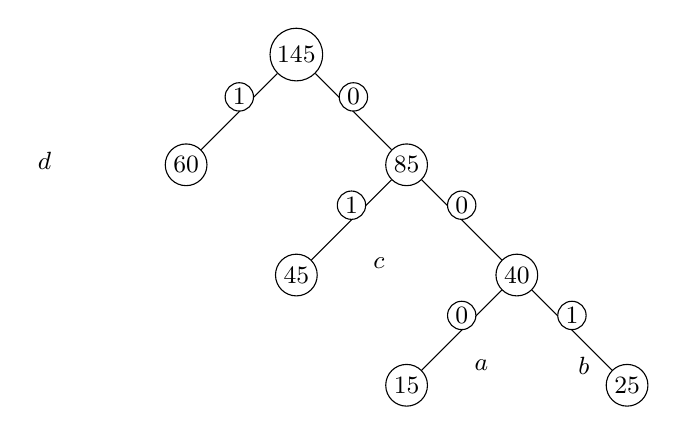
\begin{tikzpicture}[
  level distance=14mm,
  sibling distance=28mm,
  every node/.style={draw, circle, inner sep=1.5pt, font=\small},
  edge from parent/.style={draw,-},
  lab/.style={midway, fill=white, inner sep=1pt, font=\small}
]
\node {145}
  child { node {60}
    child[missing]
    child[missing]
  edge from parent node[lab, above] {1}
  }
  child { node {85}
    child { node {45}
      child[missing]
      child[missing]
      edge from parent node[lab, above] {1}
    }
    child { node {40}
      child { node {15}
        child[missing]
        child[missing]
        edge from parent node[lab, above] {0}
      }
      child { node {25}
        child[missing]
        child[missing]
        edge from parent node[lab, above] {1}
      }
      edge from parent node[lab, above] {0}
    }
    edge from parent node[lab, above] {0}
  };

% 给叶子加标签(把频率对应到字符)
\node[draw=none, font=\small] at (-3.2,-1.35) {$d$};
\node[draw=none, font=\small] at (1.05,-2.65) {$c$};
\node[draw=none, font=\small] at (2.35,-3.95) {$a$};
\node[draw=none, font=\small] at (3.65,-3.95) {$b$};
\end{tikzpicture}
\end{center}

由上图(取左边为 0、右边为 1)可给出一组编码:
$d:1,c:01,a:000,b:001.$

\noindent\textbf{(3)给出哈夫曼编码的计算复杂度(假设共有 $n$ 个字符)。}

常用实现是使用\textbf{最小优先队列(小根堆)}维护当前权值最小的两棵树:
\begin{itemize}
  \item 初始化将 $n$ 个权值入堆:$O(n)$(或 $O(n\log n)$,视建堆方式而定)。
  \item 共进行 $n-1$ 次合并,每次需要两次取最小(extract-min)和一次插入(insert):
        每次为 $O(\log n)$。
\end{itemize}

因此总时间复杂度为:$T(n)=O(n\log n).$
需要存储结点与堆结构,空间复杂度为:$S(n)=O(n).$

\noindent\textbf{(4)证明:存在 $M$ 的哈夫曼编码使 $x$ 和 $y$ 具有相同码长且仅最后一位编码不同。}

设 $x$ 和 $y$ 是 $M$ 中出现频率最小的两个字符,即 $f(x)$ 与 $f(y)$ 为最小的两个频率。
考虑任意一棵最优前缀码树(哈夫曼树) $T$。

\textbf{(a) 叶子中最深的两个结点必为兄弟:}
在二叉前缀码树中,最深层至少有两个叶子。
取最深层的两个叶子结点 $u,v$。
若 $u,v$ 不是兄弟,则可在树中进行局部交换,使得某些路径长度缩短而不破坏前缀性质,
从而不增大加权路径长度;因此总存在一棵同样最优的树,使得最深的两个叶子互为兄弟。

\textbf{(b) 最小频率字符可放在最深兄弟叶子上:}
在最优树中,若某最深叶子对应的字符频率不是最小的,
则与频率更小的字符叶子交换位置会使加权路径长度$
\sum_{m\in M} f(m)\cdot \ell(m)$
不增大(因为更小的 $f(m)$ 乘以更大的深度更“划算”)。
因此,存在一棵最优树,使得频率最小的两个字符 $x,y$ 位于最深层的两个兄弟叶子上。

由于兄弟叶子深度相同,所以 $x$ 与 $y$ 的码长相同;
又因为它们共享同一父结点,从父结点到两个叶子的最后一条边分别标记为 $0$ 与 $1$,
故它们的编码\textbf{仅最后一位不同}。

\clearpage
\subsection{回溯法}

\noindent\textbf{1. 4皇后问题:}在 $4\times 4$ 的棋盘上摆放四个皇后,使其不能互相攻击,即任意两个皇后都不能处于同一行、同一列或同一斜线上。  
\begin{enumerate}
  \item [(1)]请基于回溯法设计本问题的解向量;
  \item [(2)]给出搜索的剪枝策略,并画出解空间树;
  \item [(3)]写出基于 C/C++ 的算法伪代码;
  \item [(4)]分析所写算法的时间复杂性。
\end{enumerate}

\noindent\textbf{解答:}

\noindent\textbf{(1)解向量:}
给棋盘上的行和列分别从 1 到 4 编号,同时也给皇后从 1 到 4 编号。由于每一个皇后应该放在不同的行上,不失一般性,假设皇后 $i$放在第 $i$ 行上。
因此,4 皇后问题可以表示成一个 4 元组$(x_1, x_2, x_3, x_4),$其中 $x_i \ (i=1,2,3,4)$ 表示第 $i$ 个皇后所放置的列号。

\noindent\textbf{(2)解空间树:}
约束条件 1:当 $i \neq j$ 时,$x_i \neq x_j$;约束条件 2:当 $i \neq j$ 时,
$|x_i - x_j| \neq |i - j|$

\begin{center}
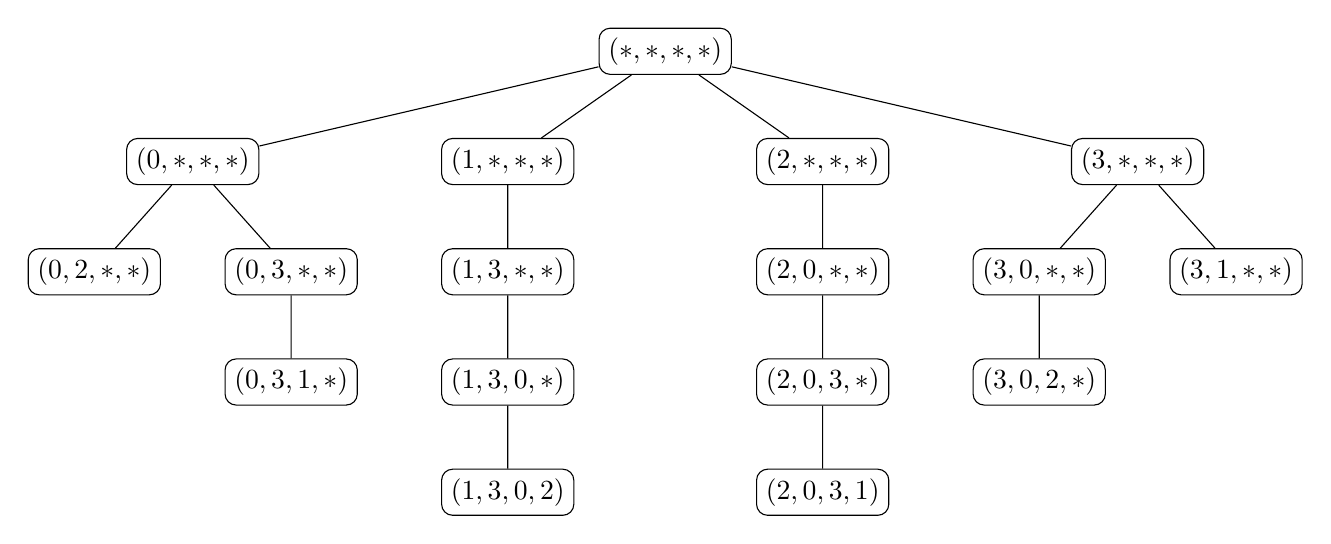
\begin{tikzpicture}[
  level 1/.style={sibling distance=40mm},
  level 2/.style={sibling distance=25mm},
  level 3/.style={sibling distance=18mm},
  level 4/.style={sibling distance=14mm},
  level distance=14mm,
  every node/.style={draw, rounded corners, align=center}
]

\node {$(\ast,\ast,\ast,\ast)$}
  child { node {$(0,\ast,\ast,\ast)$}
    child { node {$(0,2,\ast,\ast)$}
    }
    child { node {$(0,3,\ast,\ast)$}
      child { node {$(0,3,1,\ast)$}
      }
    }
  }
  child { node {$(1,\ast,\ast,\ast)$}
    child { node {$(1,3,\ast,\ast)$}
      child { node {$(1,3,0,\ast)$}
        child { node {$(1,3,0,2)$} }
      }
    }
  }
  child { node {$(2,\ast,\ast,\ast)$}
    child { node {$(2,0,\ast,\ast)$}
      child { node {$(2,0,3,\ast)$}
        child { node {$(2,0,3,1)$} }
      }
    }
  }
  child { node {$(3,\ast,\ast,\ast)$}
    child { node {$(3,0,\ast,\ast)$}
      child { node {$(3,0,2,\ast)$} }
    }
    child { node {$(3,1,\ast,\ast)$} }
  };

\end{tikzpicture}
\end{center}

\noindent\textbf{(3)代码:}
\begin{lstlisting}[language=C,style=codeStyle]
#include <iostream>
#include <math.h>
using namespace std;
int n = 8;      // 若做 4 皇后可改为 n=4
int total = 0;
int *c = new int[n];   // c[row] 表示第 row 行皇后所在列
bool is_ok(int row)
{
    for (int j = 0; j < row; j++)
    {
        // 同列:c[row] == c[j]
        // 同对角线:row + c[row] == j + c[j]
        // 同反对角线:row - c[row] == j - c[j]
        if (c[row] == c[j] ||
            row + c[row] == j + c[j] ||
            row - c[row] == j - c[j])
            return false;
    }
    return true;
}
void queen(int row)
{
    if (row == n)
        total++;
    else
    {
        for (int col = 0; col < n; col++)
        {
            c[row] = col;
            if (is_ok(row))
                queen(row + 1);
        }
    }
}
int main()
{
    queen(0);
    cout << total;
    return 0;
}
\end{lstlisting}

\noindent\textbf{(4)时间复杂度分析:}
设棋盘规模为 $n\times n$。
在回溯算法中,第 $row$ 行最多尝试 $n$ 个列位置,
每次尝试需要调用一次合法性检测函数 \texttt{is\_ok}。
该函数需要将当前皇后与之前已放置的 $row$ 个皇后进行比较,
其时间复杂度为 $O(row)$,最坏情况下为 $O(n)$。
在最坏情况下,回溯搜索树的结点数上界为
$n \cdot (n-1) \cdot (n-2) \cdots 1 = n!$
因此,算法的时间复杂度为$
T(n)=O(n\cdot n!)$

\noindent\textbf{空间复杂度分析:}
算法使用一个长度为 $n$ 的数组保存解向量,
同时递归调用的最大深度为 $n$,
因此空间复杂度为$S(n)=O(n).$

\noindent\textbf{2. 旅行售货员问题:}
某售货员要到若干城市去推销商品,已知各城市之间的路程(如下无向图所示)。
他要选定一条从驻地(城市 1)出发,经过每个城市一次,最后回到驻地的路线,使总的路程(或总旅行费)最小。
\begin{figure}[H]
  \centering
  \includegraphics[width=0.3\textwidth]{5-1-1.jpg}
\end{figure}

\begin{enumerate}
  \item [(1)]求解最优路线及其长度。
  \item [(2)]给出界限函数的设计以及求解过程中所采用的剪枝策略。
  \item [(3)]画出搜索空间树,标明发生剪枝的节点,以及树中的各个中间节点
        所对应的路径长度。
\end{enumerate}

\noindent\textbf{(1)最优解:}
最优路线为:$1 \rightarrow 3 \rightarrow 5 \rightarrow 4 \rightarrow 2 \rightarrow 1,$
其路径总长度为:16.

\noindent\textbf{(2)界限函数与剪枝策略:}

采用分支限界法求解。
设当前路径为部分路径 $P$,其已产生的路径长度为
$
\sum_{i=1}^{k-1} c(p_i,p_{i+1}),$

则其下界函数可设计为:
$
lb = \sum_{i=1}^{k-1} c(p_i,p_{i+1})
     + \sum_{v \in U} \frac{\min c(v)}{2},
$
其中 $U$ 为尚未访问的城市集合,
$\min c(v)$ 表示与城市 $v$ 相连的最小边权。
当某一结点的下界值不小于当前已知最优解时,则对该结点进行剪枝,不再继续扩展。

\noindent\textbf{(3)解空间树:}
\begin{figure}[htbp]
  \centering
  \includegraphics[width=0.9\textwidth]{5-1-2.jpg}
\end{figure}

\noindent\textbf{3.码头装箱问题:}
码头上有 $n$ 个集装箱要装上一艘载重量为 $C$ 的轮船,
其中集装箱 $i$ 的重量为 $w_i$,
请采用回溯法设计一个最优的装载方案,
即从全体集装箱中选取集装箱将该轮船尽可能地装满,
使得所装集装箱重量之和最接近 $C$。该问题等价于:
$$\max \sum_{i=1}^{n} w_i x_i$$
$$\text{s.t.}\ \sum_{i=1}^{n} w_i x_i \le C$$
$$x_i \in \{0,1\},\ 1 \le i \le n$$

\begin{enumerate}
  \item[(1)] 设集装箱的数量 $n=4$,
  轮船的载重量 $C=70$,
  每个集装箱的重量
  $W=\{30,50,20,10\}$,
  请给出本问题的解向量,
  并画出解空间树;
  \item[(2)] 给出搜索的剪枝策略;
  \item[(3)] 写出基于 C/C++ 的算法伪代码;
  \item[(4)] 分析所写算法的时间复杂性。
\end{enumerate}

\noindent\textbf{(1)解向量与解空间树:}

解向量定义为$
x=(x_1,x_2,\dots,x_n),$
其中
$
x_i=
\begin{cases}
1,& \text{选择装入第 } i \text{ 个集装箱};\\
0,& \text{不装入第 } i \text{ 个集装箱}.
\end{cases}
$

本题 $n=4, C=70, W=\{30,50,20,10\}$。

枚举可行装载中使总重量最大且不超过 $C$ 的方案:
$30+20+10=60,\quad 50+20=70,\quad 50+10=60,\quad 30+50=80(>70).$
其中最优为$50+20=70,$
对应解向量为$\boxed{x=(0,1,1,0)}.$

\begin{center}
\begin{forest}
for tree={
  draw, rounded corners, align=center,
  font=\scriptsize, inner sep=2pt,
  edge={-}, parent anchor=south, child anchor=north,
  l sep=10mm, s sep=12mm
}
[
  {(*,*,*,*)\\ cw=0}
  [
    {(1,*,*,*)\\ x1=1\\ cw=30}
    [
      {(1,1,*,*)\\ x2=1\\ cw=80}
      [{$\times$\\ OVER}, draw=none]
    ]
    [
      {(1,0,*,*)\\ x2=0\\ cw=30}
      [
        {(1,0,1,*)\\ x3=1\\ cw=50}
        [
          {(1,0,1,1)\\ x4=1\\ cw=60}
        ]
        [
          {(1,0,1,0)\\ x4=0\\ cw=50}
          [{$\times$\\ BOUND}, draw=none]
        ]
      ]
      [
        {(1,0,0,*)\\ x3=0\\ cw=30}
        [{$\times$\\ BOUND}, draw=none]
      ]
    ]
  ]
  [
    {(0,*,*,*)\\ x1=0\\ cw=0}
    [
      {(0,1,*,*)\\ x2=1\\ cw=50}
      [
        {(0,1,1,*)\\ x3=1\\ cw=70}
        [
          {(0,1,1,1)\\ x4=1\\ cw=80}
          [{$\times$\\ OVER}, draw=none]
        ]
        [
          {(0,1,1,0)\\ x4=0\\ cw=70},
          double
        ]
      ]
      [
        {(0,1,0,*)\\ x3=0\\ cw=50}
        [{$\times$\\ BOUND}, draw=none]
      ]
    ]
    [
      {(0,0,*,*)\\ x2=0\\ cw=0}
      [{$\times$\\ BOUND}, draw=none]
    ]
  ]
]
\end{forest}
\end{center}


\noindent\textbf{(2)搜索的剪枝策略:}
采用上界剪枝。设当前已装重量为 $cw$,当前最优可行解重量为 $bestw$,
剩余未处理集装箱重量之和为 $r$。
\begin{itemize}
  \item \textbf{约束剪枝:}若 $cw+w[i]>C$,则左子树(装入第 $i$ 个集装箱)不可行,直接剪去;
  \item \textbf{界限剪枝:}若 $cw+r\le bestw$,则即使把剩余所有集装箱都装入也不可能超过当前最优值,
        因此右子树(不装第 $i$ 个集装箱)可剪枝。
\end{itemize}

\noindent\textbf{(3)基于 C/C++ 的算法伪代码:}

\begin{lstlisting}[language=C,style=codeStyle]
void backtrack(int i)
{
    if (i > n) {            // 到达叶结点
        bestw = cw;         // 更新最优解
        return;
    }
    r -= w[i];              // 更新剩余重量
    if (cw + w[i] <= c) {   // 搜索左子树(装第 i 个)
        x[i] = 1;
        cw += w[i];
        backtrack(i + 1);
        cw -= w[i];
    }
    if (cw + r > bestw) {   // 搜索右子树(不装第 i 个)
        x[i] = 0;
        backtrack(i + 1);
    }
    r += w[i];              // 回退到上一层
}
\end{lstlisting}

\noindent\textbf{(4)时间复杂性分析:}
最坏情况下,回溯需要遍历所有解空间结点,
每个集装箱都有“装/不装”两种选择,因此结点数为 $2^n$ 量级。
剪枝只能减少实际搜索量,但不改变最坏情况上界。

因此该算法最坏时间复杂度为:$\boxed{O(2^n)}.$
递归深度为 $n$,并使用长度为 $n$ 的数组保存解向量,
空间复杂度为:$\boxed{O(n)}.$

\noindent\textbf{4.旅行商问题(TSP):}针对旅行商 TSP 问题,
\begin{enumerate}
  \item[(1)]采用 C/C++/Java/Python 语言伪代码,
  写出采用回溯法求解该问题的递归或非递归算法,
  同时:
  \begin{enumerate}
    \item[(i)] 设计采用的界限函数;
    \item[(ii)] 说明回溯过程中对结点采用的剪枝策略。
  \end{enumerate}
  \item[(2)] 针对下面无向图,
  以结点 1 为起始城市,
  用上述算法求解:
  \begin{enumerate}
    \item[(i)] 一条最短回路及其长度;
    \item[(ii)] 画出回溯搜索过程中生成的解空间树,
    说明发生剪枝的结点,
    以及树中各个叶结点、非叶结点对应的路径长度。
  \end{enumerate}
\end{enumerate}

\begin{figure}[H]
  \centering
  \includegraphics[width=0.3\textwidth]{5-2.png}
\end{figure}

\noindent\textbf{解答:}
\noindent\textbf{(1)回溯算法伪代码、界限函数与剪枝策略:}

\noindent\textbf{(1-i)界限函数:}
设当前已确定的部分路径为
$1=x_1 \rightarrow x_2 \rightarrow \cdots \rightarrow x_{i-1},$
其当前路径长度为 $cc$。
则对任一候选扩展 $x_i=x_j$(从未访问集合中选)时,
\textbf{下界(界限函数)}可取为$LB = cc + a[x_{i-1}][x_j].$
因为后续还要继续走若干边,总代价一定不小于已发生的代价(加上当前准备走的这一步)。

\noindent\textbf{(1-ii)剪枝策略:}
设当前已知最优回路长度为 $bestc$。
当扩展到候选结点 $x_j$ 时,若
$cc + a[x_{i-1}][x_j] \ge bestc,$
则即使继续向下搜索也不可能得到更优解,因此剪枝,不再递归该分支。

\noindent\textbf{伪代码:}
\begin{lstlisting}[language=C++,style=codeStyle]
template<class Type>
void Traveling<Type>::Backtrack(int i)
{
    if (i == n) {
        if (a[x[n-1]][x[n]] != NoEdge &&
            a[x[n]][x[1]] != NoEdge &&
            (cc + a[x[n-1]][x[n]] + a[x[n]][x[1]] < bestc
             || bestc == NoEdge)) {
            bestc = cc + a[x[n-1]][x[n]] + a[x[n]][x[1]];
        }
    }
    else
        for (int j = i; j <= n; j++) {
            if (a[x[i-1]][x[j]] != NoEdge &&
                (cc + a[x[i-1]][x[j]] < bestc
                 || bestc == NoEdge)) {
                swap(x[i], x[j]);
                cc += a[x[i-1]][x[i]];
                Backtrack(i + 1);
                cc -= a[x[i-1]][x[i]];
                swap(x[i], x[j]);
            }
        }
}
\end{lstlisting}

\noindent\textbf{(2)对给定无向图(起点为 1)的求解结果:}

图中边权为:
$a_{12}=10,\ a_{13}=20,\ a_{14}=5,\ a_{23}=15,\ a_{24}=5,\ a_{34}=5.$

\noindent\textbf{(2-i)一条最短回路及其长度:}

枚举(或按回溯搜索)可得最短回路长度为
$\boxed{35}.$
例如一条最短回路为:
$
\boxed{1 \rightarrow 2 \rightarrow 3 \rightarrow 4 \rightarrow 1},
$
其长度:
$10+15+5+5 = 35.$
(其逆序回路 $1\rightarrow 4\rightarrow 3\rightarrow 2\rightarrow 1$ 也同样为 35。)

\noindent\textbf{(2-ii)回溯搜索生成的解空间树(含剪枝结点与路径长度):}

以下树按代码的搜索顺序(从小下标到大下标)展开。
结点标注“当前部分路径 / 当前累计长度 $cc$”;叶子结点标注“回路总长度”;
被剪枝分支用 $\times$ 标出(条件为 $cc+\text{下一条边}\ge bestc$ 或超越当前最优)。

\begin{center}
\begin{forest}
for tree={
  draw,
  rounded corners,
  align=center,
  font=\scriptsize,
  inner sep=2pt,
  edge={-},
  parent anchor=south,
  child anchor=north,
  l sep=10mm,
  s sep=12mm
}
[
  {start: (1)\\ cc=0}
  [
    {(1,2)\\ cc=10}
    [
      {leaf: (1,2,3,4,1)\\ total=35},
      double
    ]
    [
      {leaf: (1,2,4,3,1)\\ total=40}
    ]
  ]
  [
    {(1,3)\\ cc=20}
    [
      {$\times$\\ prune\\ (1,3,2,*)\\ cc would be 35},
      draw=none
    ]
    [
      {leaf: (1,3,4,2,1)\\ total=40}
    ]
  ]
  [
    {(1,4)\\ cc=5}
    [
      {leaf: (1,4,3,2,1)\\ total=35}
    ]
    [
      {leaf: (1,4,2,3,1)\\ total=45}
    ]
  ]
]
\end{forest}
\end{center}




\end{document}
